% !TeX program = xelatex
% =====================================================================
%  多智能体强化学习驱动的风电场协同控制 —— 组会 / 汇报 Slides
%  编译：xelatex introduction_slides.tex （跑两次以生成目录/页码）
%  依赖：ctexbeamer（TeXLive / CTeX 均自带），需 XeLaTeX
%
%  Overleaf：上面那行 magic comment 会强制用 XeLaTeX；若仍报错，先确认
%  Menu -> Compiler 是 XeLaTeX，且 figs/ 整个目录已随 .tex 一起上传。
%  ctexbeamer 在 Overleaf 上走 Fandol 字体，不要加 fontset=windows。
% =====================================================================
\documentclass[aspectratio=169,11pt,UTF8]{ctexbeamer}

\usetheme{Madrid}
\usecolortheme{whale}
\setbeamertemplate{navigation symbols}{}
\setbeamertemplate{caption}[numbered]
\setbeamercovered{transparent}

\usepackage{amsmath,amssymb,amsfonts,mathtools}
\usepackage{bm}
\usepackage{booktabs}
\usepackage{array}
\usepackage{tikz}
\usetikzlibrary{arrows.meta,positioning,shapes.geometric,calc}
\usepackage{graphicx}

% ---- 颜色 ----
\definecolor{myblue}{RGB}{20,80,140}
\definecolor{myred}{RGB}{170,40,40}
\definecolor{mygreen}{RGB}{30,110,70}
\definecolor{mygray}{RGB}{90,90,90}
\setbeamercolor{structure}{fg=myblue}

% ---- 记号 ----
\newcommand{\R}{\mathbb{R}}
\newcommand{\E}{\mathbb{E}}
\newcommand{\Prob}{\mathbb{P}}
\newcommand{\calS}{\mathcal{S}}
\newcommand{\calA}{\mathcal{A}}
\newcommand{\calO}{\mathcal{O}}
\newcommand{\calG}{\mathcal{G}}
\newcommand{\calU}{\mathcal{U}}
\newcommand{\calN}{\mathcal{N}}
\newcommand{\bpi}{\bm{\pi}}
\newcommand{\wind}{u_{\infty}}
\newcommand{\Qhat}{\widehat{Q}}
\DeclareMathOperator*{\argmax}{arg\,max}
\newcommand{\emphb}[1]{\textcolor{myred}{\textbf{#1}}}
\newcommand{\emphg}[1]{\textcolor{mygreen}{\textbf{#1}}}

% ---- 自定义“定理/定义/假设”盒（中文标签，slides 风格）----
\newenvironment{thmbox}[1]{\begin{block}{\color{myred}\bfseries 定理\,(#1)}}{\end{block}}
\newenvironment{defbox}[1]{\begin{block}{\color{myblue}\bfseries 定义\,(#1)}}{\end{block}}
\newenvironment{asmbox}[1]{\begin{block}{\color{mygreen}\bfseries 假设\,(#1)}}{\end{block}}

% ---- 标题信息 ----
\title[MARL 风电场协同控制]{多智能体强化学习驱动的风电场协同控制}
\subtitle{从部分可观理论、多尺度 $Q$-学习收敛到 WFCRL 基准实践}
\author[项目组]{项目组汇报}
\institute[]{基于 WFCRL 基准 \& 转移独立 Dec-POMDP 理论}
\date{\today}

% ---- 每章前的“叙事弧线”导航页 ----
\AtBeginSection[]{
  \begin{frame}[plain]{Pipeline}
    \small
    \begin{columns}[T]
    \column{0.98\textwidth}
    \tableofcontents[currentsection]
    \end{columns}
    \vspace{2mm}
    \begin{center}\footnotesize\color{mygray}
    理论基座\,$\longrightarrow$\,收敛保证\,$\longrightarrow$\,工程基准\,$\longrightarrow$\,
    当前实验\,$\longrightarrow$\,next step-多模态
    \end{center}
  \end{frame}
}

\begin{document}

% =====================================================================
\begin{frame}[plain]
  \titlepage
  \begin{center}\footnotesize\color{mygray}
  理论主线依据两篇理论工作,尤以\;\emph{“Locally observable cooperative systems with acyclic dependence structure”}\;为起点
  \end{center}
\end{frame}

% ---------------------------------------------------------------------
\begin{frame}{本次汇报的叙事弧线}
\begin{columns}[T]
\column{0.56\textwidth}
\small
我们把三篇文献组织成一条\emph{从理论到实践}的链条,再落到自己的实验:
\vspace{1mm}
\begin{enumerate}\setlength\itemsep{3pt}
  \item \emphb{部分可观协同问题的 RL}(理论基础)\\[-1pt]
        {\footnotesize\color{mygray}Dec-POMDP $\to$ 转移独立重构 $\to$ 部分可观即马尔可夫噪声}
  \item \emphb{多尺度 $Q$-学习及其收敛}(Wind farm control)\\[-1pt]
        {\footnotesize\color{mygray}非平稳性 $\to$ 多时间尺度 $\to$ $\beta\le1-K$ 收敛 $\to$ 尾流 DAG}
  \item \emphb{WFCRL 基准}(实践指导)\\[-1pt]
        {\footnotesize\color{mygray}观测组成 $\to$ 奖励设计 $\to$ 风况模拟 $\to$ FLORIS/FAST.Farm 双后端}
  \item \emphg{我们的工作}:真 MAPPO,静态 vs 动态受控对照
  \item \emphg{展望}:多模态 VLM$+$RL 与数字孪生
\end{enumerate}
\column{0.44\textwidth}
\centering
\begin{tikzpicture}[node distance=5.2mm,every node/.style={font=\scriptsize}]
\tikzstyle{b}=[draw,rounded corners,align=center,fill=myblue!8,minimum width=30mm,inner sep=3pt]
\tikzstyle{g}=[draw,rounded corners,align=center,fill=mygreen!12,minimum width=30mm,inner sep=3pt]
\node[b](t1){\textbf{理论}\\部分可观 + TI-Dec-MDP};
\node[b,below=of t1](t2){\textbf{Q-学习}\\多尺度收敛 $\beta\le1-K$};
\node[b,below=of t2](t3){\textbf{基准}\\WFCRL(FLORIS/FAST.Farm)};
\node[g,below=of t3](t4){\textbf{我们}\\真 MAPPO 静/动对照};
\node[g,below=of t4](t5){\textbf{未来}\\VLM $+$ RL 数字孪生};
\draw[-{Latex[length=2mm]},myblue,thick](t1)--(t2);
\draw[-{Latex[length=2mm]},myblue,thick](t2)--(t3);
\draw[-{Latex[length=2mm]},mygreen,thick](t3)--(t4);
\draw[-{Latex[length=2mm]},mygreen,thick](t4)--(t5);
\end{tikzpicture}
\end{columns}
\end{frame}

% ---------------------------------------------------------------------
\begin{frame}{目录}
\tableofcontents
\end{frame}

% =====================================================================
\section{动机:尾流、协同与一个理论谜题}
% =====================================================================

\begin{frame}{风电场里的尾流问题}
\begin{columns}[T]
\column{0.6\textwidth}
\small
单台机组从风中提取动能,在其\emph{下游}留下一条\emphb{尾流(wake)}:风速降低、湍流增强。密集布置成风电场后,上游尾流“笼罩”下游机组,造成两类损失:
\begin{itemize}\setlength\itemsep{3pt}
  \item \emphb{发电损失}:可用风功率 $\propto u^3$,大型海上风场整场功率损失可达 \textbf{10\%--20\%};
  \item \emphb{疲劳加剧}:高湍流使下游叶片/塔筒承受更强交变载荷,疲劳上升 \textbf{5\%--15\%}。
\end{itemize}
\vspace{1mm}
\emphg{尾流偏转控制(wake steering)}:上游机组\emph{主动偏航}少发一点电,把尾流\emph{侧向偏转}离开下游 —— 牺牲局部、成全整场。这是本研究的核心控制手段。
\column{0.4\textwidth}
\centering
\begin{tikzpicture}[scale=0.9,every node/.style={font=\scriptsize}]
% 贪心
\node[font=\scriptsize\bfseries] at (1.6,2.5){贪心:对准来流};
\fill[myblue!12] (0,1.4) rectangle (3.2,2.2);
\draw[very thick] (0.4,1.4)--(0.4,2.2); % T1 rotor
\draw[myred!70,-{Latex[length=1.5mm]}] (0.5,1.8)--(2.2,1.8);
\draw[very thick] (2.3,1.5)--(2.3,2.1); % T2 in wake
\node at (0.4,1.25){\tiny 上游};
\node at (2.3,1.25){\tiny 下游(尾流中)};
% steering
\node[font=\scriptsize\bfseries] at (1.6,0.7){尾流偏转:偏航};
\fill[mygreen!14] (0,-0.9) rectangle (3.2,0.3);
\draw[very thick,rotate around={25:(0.4,-0.3)}] (0.4,-0.6)--(0.4,0.0);
\draw[mygreen!60,-{Latex[length=1.5mm]}] (0.5,-0.3) .. controls (1.4,-0.1) and (1.9,0.25) .. (2.6,0.28);
\draw[very thick] (2.3,-0.6)--(2.3,0.0);
\node at (2.3,-1.05){\tiny 下游(尾流偏开)};
\end{tikzpicture}
\end{columns}
\end{frame}

% ---------------------------------------------------------------------
\begin{frame}{尾流偏转:FLORIS 真实算例(\texttt{Turb3\_Row1})}
\begin{center}
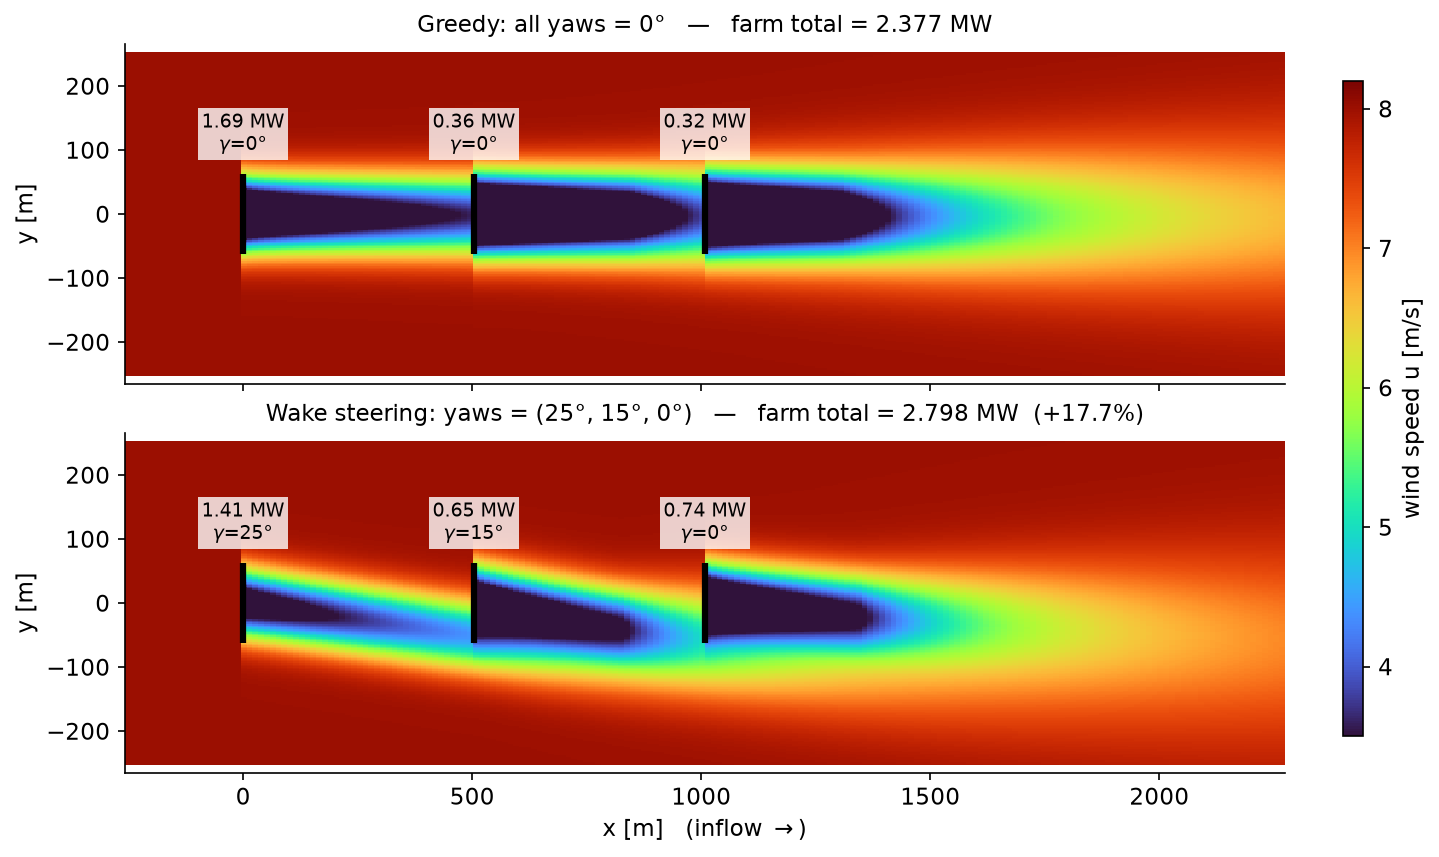
\includegraphics[width=0.83\textwidth]{figs/fig_wake_steering.png}
\end{center}
\vspace{-2mm}
\footnotesize
三机组沿来流方向以 $4D$($504$\,m,$D=126$\,m)对齐,$\wind=8$\,m/s —— \emph{尾流效应最显著的最坏布局}。
\begin{itemize}\setlength\itemsep{1pt}
  \item \textbf{贪心}(全部对准来流):下游两台深陷尾流,功率只有 $0.36$ / $0.32$\,MW,\emph{不到上游的四分之一};
  \item \textbf{尾流偏转}:上游牺牲 $1.69\!\to\!1.41$\,MW,把尾流侧向推开,下游\emph{几乎翻倍}($0.65$/$0.74$\,MW);
  \item 整场 $2.377\!\to\!2.798$\,MW,\emphb{$+17.7\%$} —— 这就是协同控制要抓的收益。
\end{itemize}
\end{frame}

% ---------------------------------------------------------------------
\begin{frame}{协同问题的真实面貌:非凸、多峰、贪心解在谷底}
\begin{center}
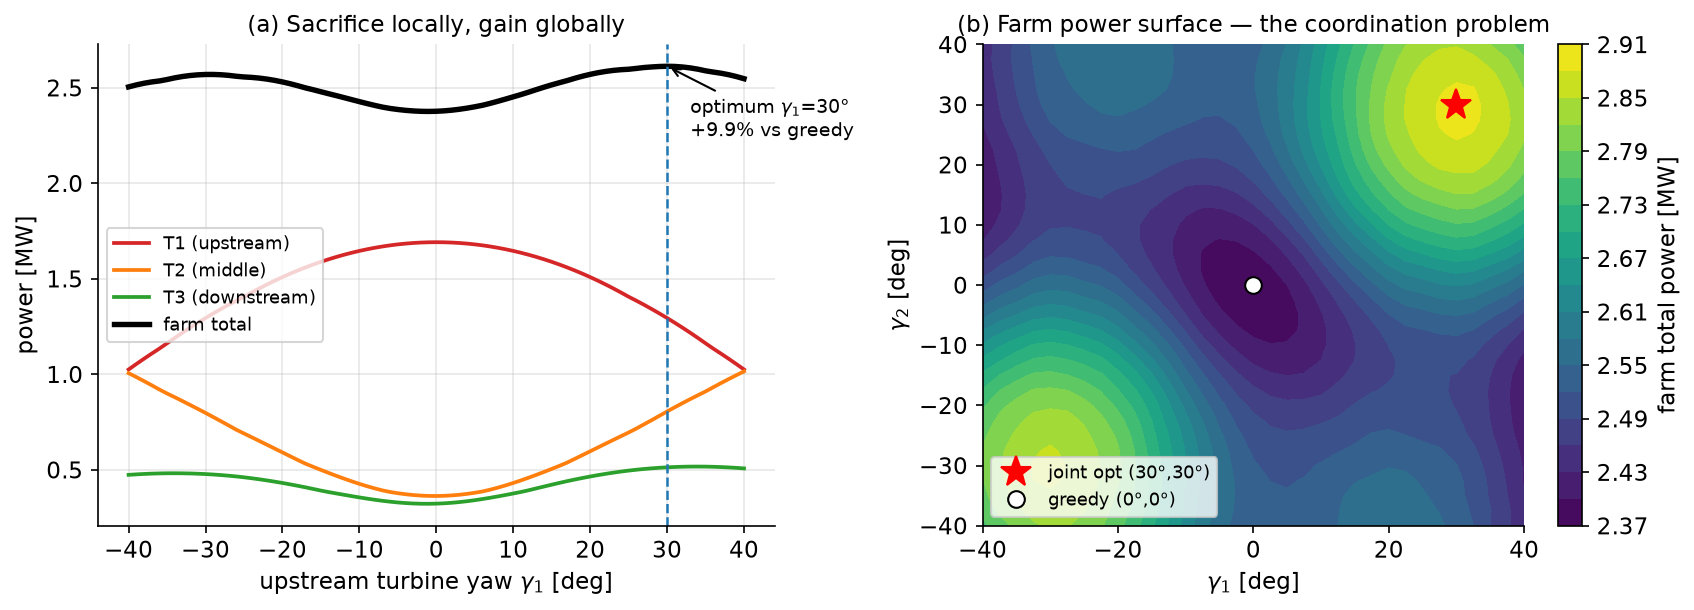
\includegraphics[width=0.95\textwidth]{figs/fig_yaw_power.png}
\end{center}
\vspace{-1mm}
\footnotesize
\begin{columns}[T]
\column{0.5\textwidth}
\textbf{(a) 牺牲局部、成全整体}\\
只调上游偏航 $\gamma_1$:$T_1$ 功率单调下降,$T_2/T_3$ 显著上升,\emph{整场}在 $\gamma_1=30^\circ$ 取最优,较贪心 \emphb{$+9.9\%$}。
\emph{贪心解 $\gamma_1=0$ 恰恰落在整场功率的局部极小点上。}
\column{0.5\textwidth}
\textbf{(b) 这才是协同的难点}\\
$(\gamma_1,\gamma_2)$ 联合功率面\emph{非凸}且有\emphb{两个对称最优}$(\pm30^\circ,\pm30^\circ)$。
$\Rightarrow$ 存在\emph{均衡选择}问题:两台机组必须\emph{一致地}选同号偏航,选反了反而更差。
\end{columns}
\vspace{1mm}
\centering\footnotesize\color{mygray}
这正呼应后面的理论:去中心化学习收敛到的是\emph{某个均衡},未必是全局最优 —— 多峰结构使这一区别具体可见。
\end{frame}

\begin{frame}{为什么必须用(多智能体)强化学习}
\small
\begin{columns}[T]
\column{0.5\textwidth}
\textbf{为什么是 RL?}\\
从全场偏航/桨距/转矩到三维风速场的映射由 \emphb{Navier--Stokes 方程}支配 —— 高维、强非线性、在线优化不可解;高保真 CFD/LES 一次要跑数小时。\\[2pt]
$\Rightarrow$ 用\emph{数据驱动的策略}逼近最优控制,而非求解显式物理模型。
\column{0.5\textwidth}
\textbf{为什么是多智能体?}\\
风电场天然是多智能体系统:每台机组是自主决策单元,只观测局部风况,通过共享尾流场耦合、共享团队目标。\\[2pt]
$\Rightarrow$ \emphg{去中心化执行}、通信开销低、随机组数可扩展;而单一中央控制器的联合动作空间随机组数\emph{指数爆炸}。
\end{columns}
\vspace{2mm}
\begin{alertblock}{贯穿全场的核心谜题(本汇报的理论主线)}
\centering
\emph{独立学习}(每台机组各跑一个单体 RL)在一般 MARL 中因\emphb{非平稳性}\textbf{没有收敛保证},\\
但在风电场上\emph{经验上却很有效}。—— \textbf{为什么?在什么条件下能保证收敛?}
\end{alertblock}
\end{frame}

% =====================================================================
\section{理论基础:部分可观协同问题的 RL}
% =====================================================================

\begin{frame}{起点:协同 Dec-POMDP 及其困难}
\small
$M$ 台机组的协同控制被建模为\emphb{去中心化部分可观马尔可夫决策过程}(Dec-POMDP):
\[
\big\{\,M,\ \calS,\ \{\calA_i\},\ P,\ \{\calO_i\},\ r\,\big\},\qquad
\calA=\textstyle\prod_i\calA_i,\ \ \calO=\prod_i\calO_i.
\]
全局状态 $s\in\calS$,转移核 $P(s,a,s')$,\emph{有界共享奖励} $|r(s,a)|\le R$。机组 $i$ 依局部历史 $h_i$ 执行随机策略 $\pi_i(a_i|h_i)$,联合策略 $\bpi(a|h)=\prod_i\pi_i(a_i|h_i)$,目标
\[
\max_{\bpi}\ \E\Big[\sum_{k\ge0}\beta^k\,r_k\Big],\qquad 0<\beta<1.
\]
\begin{itemize}\setlength\itemsep{2pt}
  \item \emphb{困难一}:使问题马尔可夫化的“真状态”是\emph{整个风场速度场},不可观 —— 只能用局部测量。
  \item \emphb{困难二}:一般 Dec-POMDP 最优规划是 \textbf{NEXP-hard};独立学习又非平稳,无收敛保证。
\end{itemize}
\centering\vspace{1mm}
\emphg{论文的破局思路:重构问题结构,把“不可观”变成可控的噪声。}
\end{frame}

\begin{frame}{关键一招:牺牲状态可观性,换取转移独立性}
\small
每台机组的局部信息可分解为两部分:
\[
\underbrace{y_i}_{\text{私有:自己的偏航}}\quad\text{和}\quad
\underbrace{w_i}_{\text{耦合:局部风况(受他人偏航影响)}}.
\]
$w_i$ 是\emph{他人动作}与\emph{外生来流}的未知函数(由 3D Navier--Stokes 决定)。\emphb{把随他人动作变化的 $w_i$,替换为对外生来流的单一共享观测 $\wind$}:
\[
\text{局部状态}\quad s_i=(y_i,\ \wind)\quad\Longrightarrow\quad \text{不再依赖其他机组的动作。}
\]
\begin{defbox}{转移独立的 Dec-POMDP(TI-Dec-MDP)}
若全局转移核可按机组分解
$\;P(s,a,s')=\prod_{i=1}^{M}P^i(s_i,a_i,s'_i)\;$,
则机组\emphb{仅通过共享奖励}耦合,且最优可由\emph{局部策略之积}达到。
\end{defbox}
\centering
\emph{“我们用状态可观性,换来了转移独立性。”} —— 代价是引入部分可观。
\end{frame}

\begin{frame}{部分可观 $=$ 状态相关的马尔可夫噪声}
\small
把 $w_i$ 换成 $\wind$ 后,机组 $i$ 看不到全局状态 $s$,只看到 $s_i$。于是从 $i$ 的视角:
\begin{itemize}\setlength\itemsep{2pt}
  \item 在固定的 $(s_i,a_i)$ 下,收到的奖励 $r$ \emph{仍会波动} —— 因为它取决于\emph{看不见}的其他机组状态 $s_{-i}$;
  \item 但 $s_{-i}$ 并非任意:在其他机组的\emph{平稳策略}下,它是一条\emphb{几何遍历}的马尔可夫链。
\end{itemize}
\begin{block}{核心观察(全文分析的支点)}
从单个学习者看,\emphb{部分可观带来的奖励偏差,是一个未观测马尔可夫过程的函数} —— 即\emph{状态相关的马尔可夫噪声},而非零均值鞅噪声。它可以\emph{被平稳分布平均掉},而不是被简单当作方差。
\end{block}
定义在平稳分布 $d_{\bpi}$ 下的\emph{局部 $Q$ 函数}
\[
Q^{\bpi_{-i}}_{\pi_i}(s_i,a_i)=\E_{s_{-i}\sim d_{\bpi_{-i}}}\!\big[\,Q^{\bpi}(s,a)\,\big],
\]
满足一条\emph{局部 Bellman 递归}(论文 Lemma 2.1)—— 这是把多智能体问题降回“单体 $Q$-学习 + 噪声”的桥梁。
\end{frame}

\begin{frame}{最优响应、光滑化与均衡}
\small
给定他人策略 $\bpi_{-i}$,机组 $i$ 的\emph{最优响应}是贪心策略 $\argmax_{a_i}Q_i(s_i,a_i)$。为保证可微与探索,用\emphb{光滑化最优响应}(温度 $\tau$,强凹正则 $\nu$):
\[
\phi_\tau(Q_i)(\cdot\,|\,s_i)\;=\;\argmax_{\rho\in\Delta(\calA_i)}\ \Big\{\ \rho^{\!\top}Q_i(s_i,\cdot)\;+\;\tau\,\nu(\rho)\ \Big\},
\]
例如 $\nu=$ 熵时即 \emph{Boltzmann/softmax} 策略。
\begin{defbox}{($\tau$-光滑)均衡}
一组局部策略 $\bpi^\star=(\pi_1^\star,\dots,\pi_M^\star)$ 称为均衡,若对每台机组
$\;\pi_i^\star=\phi_\tau\big(Q^{\bpi_{-i}^\star}_{\pi_i^\star}\big)\;$ —— 即\emph{每台机组都在对其余机组做光滑最优响应},没有机组能单方面改善。
\end{defbox}
\begin{itemize}\setlength\itemsep{1pt}
\item \textbf{目标从“求全局最优”松弛为“求均衡”}:这在去中心化、部分可观下是可达且可分析的解概念。
\item \textbf{剩下的问题}:能否用\emph{独立、异步}的 $Q$-学习迭代\emph{收敛}到这个均衡?$\to$ 下一节。
\end{itemize}
\end{frame}

% =====================================================================
\section{收敛保证:多时间尺度 $Q$-学习}
% =====================================================================

\begin{frame}{非平稳性:独立学习为何一般不收敛}
\small
若所有机组\emph{同时、同速}更新各自的 $Q_i$,则每台机组眼中的“环境”(其余机组的策略)在\emph{不断漂移} —— 目标随学随变,标准 $Q$-学习的收缩性被破坏。这就是\emphb{非平稳性}。
\vspace{1mm}
\begin{block}{解法:多时间尺度(multi-timescale)随机逼近}
让不同机组以\emph{不同的学习率量级}更新:
\[
\text{当 } i<j:\quad \frac{\alpha^i_k}{\alpha^j_k}\to 0.
\]
\emph{慢}迭代在\emph{快}迭代看来近似\emphb{静止}(于是快迭代面对的是平稳环境);\emph{快}迭代在\emph{慢}迭代看来已\emphb{收敛到均衡}(于是慢迭代面对的是已达最优响应的对手)。
\end{block}
\centering
思想源头:Borkar 双时间尺度随机逼近 $\Rightarrow$ 本文推广到 \emph{$M$ 个时间尺度} + \emph{马尔可夫噪声}。
\end{frame}

\begin{frame}{多尺度 $Q$-学习(MQL)与收敛定理}
\small
\emph{多尺度 $Q$-学习(MQL)}迭代:每台机组按自己的尺度做局部 $Q$-学习,并以光滑响应生成行为策略
\[
Q^{i}_{k+1}(s_i,a_i)=Q^{i}_{k}(s_i,a_i)+\alpha^i_k\,\Big[\,r_k+\beta\max_{a'}Q^i_k(s'_i,a')-Q^i_k(s_i,a_i)\,\Big],\quad \pi^i_k=\phi_\tau(Q^i_k).
\]
\begin{asmbox}{A3.1 · 奖励的 Lipschitz 收缩}
存在机组排序与常数 $K\in(0,1)$,使某机组值函数的局部扰动,对\emph{均衡奖励场}的影响\emph{严格更小}:
\[
\big\|\,r_{\bpi}-r_{\bpi'}\,\big\|_{\infty}\ \le\ K\,\big\|\,Q_i-Q'_i\,\big\|_{\infty}.
\]
\emph{物理含义}:沿下游方向,尾流耦合是一个\emphb{收缩} —— 上游对下游的影响不会被逐级放大。
\end{asmbox}
\begin{thmbox}{Thm 3.1 · 多尺度 $Q$-学习收敛}
在转移独立、遍历性、多尺度学习率(Robbins--Monro $\sum\alpha=\infty,\sum\alpha^2<\infty$ + 尺度分离)与 A3.1 下,\emph{若}
\[
\boxed{\ \beta\ \le\ 1-K\ }
\]
\emph{则}各机组的 $Q^i$ 弱收敛到光滑最优响应值,其诱导策略构成一个\emph{均衡}。
\end{thmbox}
\end{frame}

\begin{frame}{定理怎么证:随机逼近的 ODE 方法}
\small
这本质是一篇\emphb{随机逼近}工作。给关注随机优化的同行一座桥:
\begin{center}\renewcommand{\arraystretch}{1.25}
\begin{tabular}{@{}ll@{}}
\toprule
\textbf{单体 / SGD 直觉} & \textbf{本文多智能体对应物} \\
\midrule
$Q$-学习更新 & Robbins--Monro 迭代 \\
Bellman 算子 $\beta$-收缩 & 跨机组\emph{联合}收缩(靠时间尺度分离) \\
双时间尺度(Borkar) & \emph{$M$ 时间尺度}异步更新 \\
有界方差的零均值噪声 & \emphb{状态相关马尔可夫噪声}(部分可观) \\
收敛性 & Kushner--Yin \emph{ODE 方法} + 弱收敛 \\
噪声被平均掉 & \emph{几何遍历性} $\|d_nP^\ell-D\|_1\le C(1-b)^\ell$ \\
\bottomrule
\end{tabular}
\end{center}
\vspace{1mm}
\begin{itemize}\setlength\itemsep{2pt}
  \item 关键难点:噪声\emph{不是}零均值鞅,而是未观测链的函数 $\Rightarrow$ 经典 Robbins--Monro 不直接适用;
  \item 解决:多尺度让快变量“就地”平衡马尔可夫噪声,慢变量只看到其\emph{平均} ODE $\Rightarrow$ 逐尺度归纳收敛。
\end{itemize}
\end{frame}

\begin{frame}{利用尾流结构:DAG 与 NetworkMQL}
\small
\begin{columns}[T]
\column{0.55\textwidth}
在给定来流方向下,能量\emph{只向下游流动} $\Rightarrow$ “$i$ 的尾流影响 $j$”构成\emphb{有向无环图(DAG)} $\calG=(V,E)$。“无环”只禁止\emph{有向回路},\emphb{不禁止多父节点}——一台机组常同时处于多台上游机组的\emph{叠加尾流}中。据此奖励可\emph{分解}:
\[
r(s,a)=\sum_{i=1}^{M}r_i\big(s_i,a_i,\ s_{\calU_i},a_{\calU_i}\big),\quad \calU_i=\calN^i_{\mathrm{in}}
\]
即\emph{网络化分布式 POMDP}(ND-POMDP)。
\begin{thmbox}{Thm 3.2 · NetworkMQL}
若秩函数 $\mathrm{rk}:V\to\{1,\dots,\bar M\}$ 满足\\
\textbf{(A)} 任一 $i$ 的\emph{祖先}秩严格更小、\emph{后代}秩严格更大;\\
\textbf{(B)} 任一 $i$ 的\emph{祖先集内不存在两个同秩节点},\\
则 Thm 3.1 的收敛性保持,而尺度数由 $M$ 降至 \emphb{$\bar M\le M$}(e.g., 16 机组 $\to\bar M=9$)。
\end{thmbox}
\column{0.45\textwidth}
\centering
\begin{tikzpicture}[>={Latex[length=1.5mm]},every node/.style={font=\scriptsize}]
\tikzstyle{t}=[circle,draw,fill=myblue!12,minimum size=6mm,inner sep=0]
\node[t] (a1) at (0,0.7)   {$1$};
\node[t] (a2) at (0,-0.7)  {$2$};
\node[t] (a3) at (1.3,0)   {$3$};
\node[t] (b1) at (2.7,0.7) {$4$};
\node[t] (b2) at (2.7,-0.7){$5$};
\node[t] (b3) at (4.0,0)   {$6$};
\draw[->,myred] (a1)--(a3); \draw[->,myred] (a2)--(a3);
\draw[->,myred] (b1)--(b3); \draw[->,myred] (b2)--(b3);
\node[above=0.4mm of a1,text=mygreen,font=\tiny]{rk\,1};
\node[below=0.4mm of a2,text=mygreen,font=\tiny]{rk\,2};
\node[above=0.4mm of a3,text=mygreen,font=\tiny]{rk\,3};
\node[above=0.4mm of b1,text=mygreen,font=\tiny]{rk\,1};
\node[below=0.4mm of b2,text=mygreen,font=\tiny]{rk\,2};
\node[above=0.4mm of b3,text=mygreen,font=\tiny]{rk\,3};
\draw[dashed,mygray] (2.0,-1.5) -- (2.0,1.5);
\node[text=mygray,font=\tiny,align=center] at (2.0,-1.95) {两簇尾流\\互不汇合};
\draw[->,thick,mygray] (-0.9,-1.7) -- (-0.15,-1.7);
\node[text=mygray,font=\tiny] at (-0.5,-2.05) {来流};
\end{tikzpicture}
\vspace{1mm}
{\footnotesize\color{mygray} 3 号有\emph{两个}父节点(合法);但 1、2 同为 3 的祖先,由 (B) \emph{必须错开}尺度。1 与 4 无\emph{共同后代},故可同秩 $\Rightarrow$ $\bar M=3<M=6$。}
\end{columns}
\end{frame}

\begin{frame}{理论的经验验证与适用边界}
\small
\begin{columns}[T]
\column{0.54\textwidth}
\textbf{经验验证(Wind farm control 论文)}
\begin{itemize}\setlength\itemsep{2pt}
  \item 在真实的 \textbf{16 机组}风电场上,MQL / NetworkMQL \emph{经验性地收敛};
  \item 对照\emph{朴素}独立 $Q$-学习(LQL,所有机组同尺度):后者\emph{震荡/不稳},印证非平稳性诊断;
  \item 多尺度以\emph{可控的收敛速度代价},换来\emph{稳定性与收敛保证}。
\end{itemize}
\column{0.46\textwidth}
\begin{alertblock}{适用边界(与我们工作的接口)}
保证成立于:\emph{直接观测} $\wind$(转移独立)且\emph{有限表格} $Q$。一旦引入
\emphb{连续动作 / 深度函数逼近 / 含噪局部观测},前提被打破。
\end{alertblock}
\end{columns}
\vspace{1mm}
\begin{block}{承上启下}
\centering
理论给了\emph{“为什么独立学习能work”}的干净答案与充分条件 $\beta\le1-K$。\\
但真实工程要\emph{连续动作 + 深度网络 + 高保真动态} —— 这正是 \emphg{WFCRL 基准}与我们实验的出发点。
\end{block}
\end{frame}

% =====================================================================
\section{实践指导:WFCRL 基准}
% =====================================================================

\begin{frame}{WFCRL:面向风电场控制的 MARL 基准}
\small
WFCRL 把上述理论\emph{落地为可复现的实验平台}:统一的 Dec-POMDP 接口 $+$ 两种保真度物理后端 $+$ 标准基线,以 Gymnasium / PettingZoo 接口开源(Apache-2.0)。
\begin{columns}[T]
\column{0.52\textwidth}
\textbf{可选的三个维度}(环境 ID $=$ 前缀$+$根$+$后缀)
\begin{itemize}\setlength\itemsep{1pt}
  \item \emph{控制形式}:\texttt{Dec\_} 前缀 $=$ 去中心化(PettingZoo);无前缀 $=$ 集中式(Gymnasium);
  \item \emph{布局}:$3$ 机组玩具阵列 $\to$ HornsRev2($91$ 台),含 5 个真实风场;
  \item \emph{仿真器}:\texttt{\_Floris}(静态)/ \texttt{\_Fastfarm}(动态)。
\end{itemize}
\vspace{1mm}
所有机组均为 \textbf{NREL 5\,MW 参考机组}($D=126$\,m,轮毂 $90$\,m)。
\column{0.48\textwidth}
\textbf{标准基线与经验规律}
\begin{itemize}\setlength\itemsep{1pt}
  \item \emph{IPPO} / \emph{MAPPO}(CTDE)/ \emph{QMIX} / \emph{IDRQN};
  \item 小规模($3$ 机组):IPPO 常占优;
  \item $7$ 机组以上:MAPPO 共享 critic 优势显现;
  \item 来流越多样,\emph{信息共享越有价值};
  \item 在 FAST.Farm 上,\emph{局部风观测被他机湍流扰动},只在 Sc.\,I 训练的 IPPO 明显吃亏。
\end{itemize}
\end{columns}
\vspace{1mm}
\centering\footnotesize\color{mygray}
下面三页依次展开:\textbf{观测量的组成}、\textbf{奖励函数的设计}、\textbf{风况的模拟原理}。
\end{frame}

% ---------------------------------------------------------------------
\begin{frame}{(一)观测量的组成}
\small
\textbf{出发点}:能让系统马尔可夫化的“真状态”是\emph{整个风场的三维速度场} —— 实际不可知。WFCRL 因此只假设\emph{每台机组有局部风速/风向测量},外加一个\emph{自由来流估计}(且不保证实时下发到各机组)。
\begin{center}\footnotesize\renewcommand{\arraystretch}{0.25}
\begin{tabular}{@{}p{0.17\linewidth} p{0.36\linewidth} p{0.40\linewidth}@{}}
\toprule
 & \textbf{FLORIS(静态)} & \textbf{FAST.Farm(动态)} \\
\midrule
局部观测 $o^i$ & $u_i,\ \phi_i$(\emph{稳态}值),$y_i$ & $u_i,\ \phi_i$(\emph{时变}),$y_i,\ p_i,\ \tau_i$ \\
全局观测 $o_g$ & \multicolumn{2}{c}{$(o^1,\dots,o^M,\ \wind,\ \phi_\infty)$ —— 各局部观测拼接 $+$ 自由来流} \\
动作 & $\Delta y_i$ & $\Delta y_i,\ \Delta p_i,\ \Delta \tau_i$ \\
\bottomrule
\end{tabular}
\end{center}
\footnotesize
\begin{columns}[T]
\column{0.52\textwidth}
\textbf{我们实际用的空间}(\texttt{Dec\_Turb3\_Row1\_Floris} 实测)
\begin{itemize}\setlength\itemsep{0pt}
  \item \texttt{yaw}: \texttt{Box(-40, 40, (1,))} — 偏航\emph{绝对角}上下界 $\pm40^\circ$
  \item \texttt{wind\_speed}: \texttt{Box(3, 28, (1,))}
  \item \texttt{wind\_direction}: \texttt{Box(0, 360, (1,))}
  \item 动作 \texttt{yaw}: \texttt{Box(-5, 5, (1,))} — \emphb{增量}
  \item 全局另附 \texttt{freewind\_measurements}: $(\wind,\phi_\infty)$
\end{itemize}
\column{0.48\textwidth}
\begin{block}{三个设计要点}
\footnotesize
\begin{enumerate}\setlength\itemsep{1pt}
  \item \emph{为什么含 $\theta_i$(执行器上一步目标)}:FAST.Farm 的执行器内环有\emph{响应时延},下发目标 $\neq$ 当前实际值;FLORIS 上二者恒等。
  \item \emph{为什么动作是增量}:真实偏航有\emph{速率上限},只能渐变;上下界即物理速率约束。
  \item \emph{与理论的接口}:理论把 $o^i$ 里的\emph{局部}风 $u_i$ 换成\emph{全场共享}的 $\wind$,才换来转移独立 —— 基准保留 $u_i$,所以\emph{更真实但也更难}。
\end{enumerate}
\end{block}
\end{columns}
\end{frame}

% ---------------------------------------------------------------------
\begin{frame}{(二)奖励函数的设计}
\small
\begin{columns}[T]
\column{0.53\textwidth}
\textbf{功率项}(整场功率,按机组平均、按来流立方归一化)
\[
r^{P}_{k}=\frac{1}{M}\sum_{i=1}^{M}\frac{\widehat P^{\,i}_{k}}{(u_{\infty,k})^{3}}
\]
\textbf{载荷项}。FLORIS \emph{无}结构模型,用流场\emph{代理}(转子平面 $9$ 点网格上的湍流强度 $+$ 三向速度标准差):
\[
r^{L}_{k,S}=\frac{1}{M}\sum_{i}\Big(\sum_{j=1}^{9}TI_k[x_{i,j}]+\sigma(u_k)+\sigma(v_k)+\sigma(w_k)\Big)
\]
FAST.Farm 用\emph{真实}叶片弯矩(面外 op $+$ 面内 ip,每台 3 叶片):
\[
r^{L}_{k,D}=\frac{1}{M}\sum_{i}\Big(\sum_{j=1}^{3}|M^{\text{op}}_k[i,j]|+\sum_{j=1}^{3}|M^{\text{ip}}_k[i,j]|\Big)
\]
\textbf{合成}:$\;r_k=r^{P}_k-\alpha\,r^{L}_k$,默认 $\alpha=1$(两项已缩放到同量级)。
\column{0.47\textwidth}
\begin{block}{此外还有一条硬约束}
\footnotesize 执行器\emph{占空比}:每台机组用于偏航动作的\emph{时间}不得超过 $10\%$。每步计算所需动作时间,\emph{违反则该动作被置零} —— 所以训练时看到偏航“卡住”是正常的。
\end{block}
\vspace{-1mm}
\begin{alertblock}{为什么要除以 $\wind^3$}
\footnotesize 风功率 $\propto u^3$。不归一化,奖励几乎完全由\emph{风大风小}决定,\emph{淹没}了控制质量的信号。见下页图 (a):原始功率在 $u_\infty\!\in\![4,12]$ 内变化 \textbf{$40$ 倍},而 $r^P$ 基本持平。
\end{alertblock}
\end{columns}
\end{frame}

% ---------------------------------------------------------------------
\begin{frame}{(二)奖励设计的两个实证检验}
\begin{center}
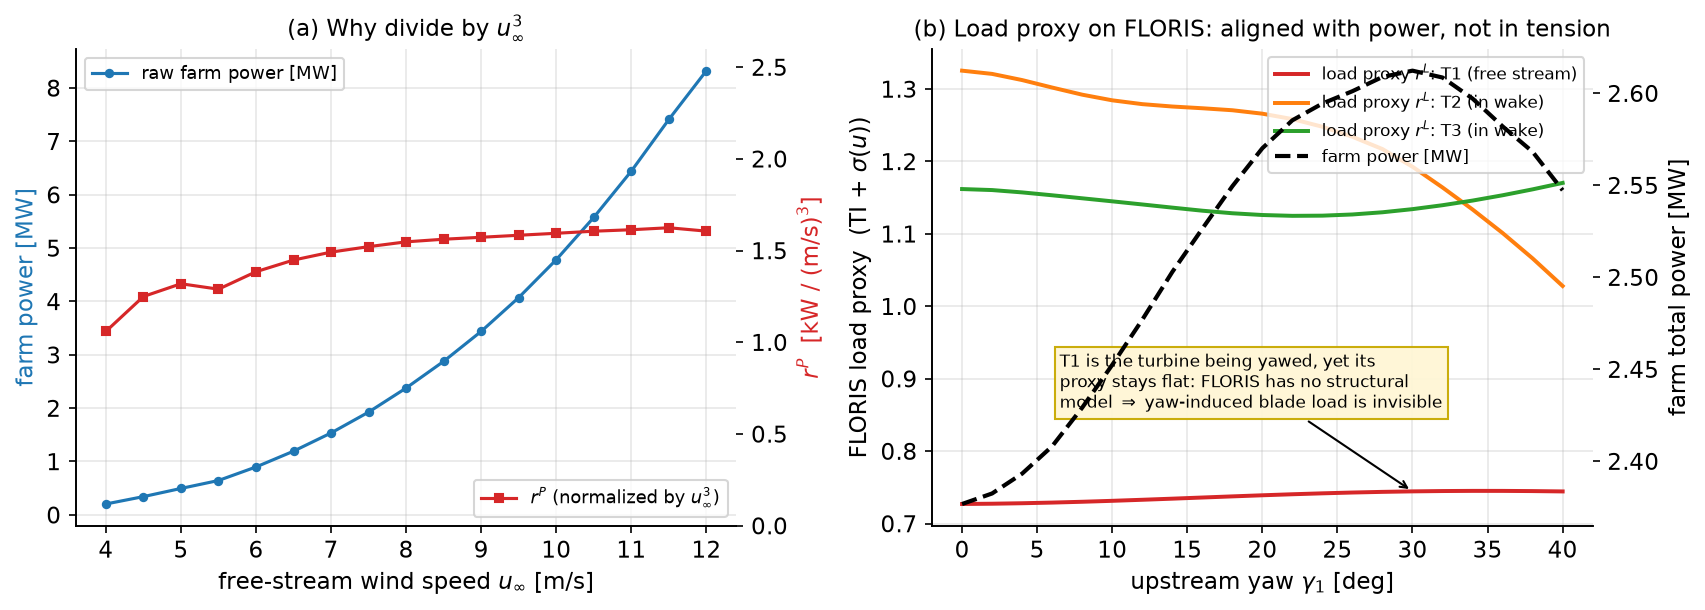
\includegraphics[width=0.75\textwidth]{figs/fig_reward_design.png}
\end{center}
\vspace{-1mm}
\footnotesize
\begin{columns}[T]
\column{0.4\textwidth}
\textbf{(a) 立方归一化确实起作用}\\
原始整场功率随 $\wind$ 从 $0.2$ 涨到 $8.3$\,MW($\sim\!40\times$);归一化后的 $r^P$ 只在 $1.0\!\sim\!1.6$ 间小幅变化 $\Rightarrow$ 学习信号\emph{反映控制质量而非风况}。
\column{0.52\textwidth}
\textbf{(b) 一处局限}\\
FLORIS 的载荷是\emph{纯流场}的:被偏航的 $T_1$ 自身deg值\emph{几乎不变}(红线),因为 FLORIS \emph{没有结构模型},看不见偏航引起的叶片交变载荷。于是在 FLORIS 上\emphb{功率与载荷代理是同向的},$\alpha$ 几乎不改变最优解。
\emphg{真正的功率—疲劳张力,只有在 FAST.Farm 的真实弯矩上才会出现} —— 这也是我们必须上动态后端的理由之一。
\end{columns}
\end{frame}

% ---------------------------------------------------------------------
\begin{frame}{(三)风况的模拟原理}
\small
风况是这个问题里唯一的\emph{外生随机源}(理论中那个“可观测的外生马尔可夫过程”)。WFCRL 定义三种场景,区别在于\emph{随机性在什么时间尺度上进入}:
\begin{columns}[T]
\column{0.55\textwidth}
\begin{itemize}\setlength\itemsep{2pt}
  \item \textbf{场景 I}:全程固定在该风场的\emph{主导}风速与风向 $\Rightarrow$ 检验\emph{纯协同}能力,无分布迁移。
  \item \textbf{场景 II}:\emph{每回合开始}重采样自由来流
  \[
    \wind\sim\mathcal W(\bar u,\lambda),\qquad \phi_\infty\sim\mathcal N(\bar\phi,\sigma_\phi)
  \]
  Weibull 是风速的标准工程分布($\lambda$ 形状、$\bar u$ 尺度),风向用绕主导风向的正态 $\Rightarrow$ 检验\emph{跨风况泛化}。
  \item \textbf{场景 III}:回合\emph{内}来流随时间变化,回放真实风场实测序列,每回合随机选起点 $\Rightarrow$ 最接近现场。
\end{itemize}
\column{0.45\textwidth}
\begin{block}{评价分数(场景 II)}
\footnotesize
\[
\text{score}=\sum_{j=1}^{n_w}\rho_j\sum_{k=0}^{T}r_k,\qquad \sum_j\rho_j=1
\]
在 $n_w=25$ 组风况上按权重 $\rho_j$ 加权。$\rho_j$ 由 \textbf{SMARTEOLE} 项目在 Ablaincourt 风场的实测\emph{风况}(风速$\times$风向二维直方图)提取。
\emph{关键}:评价用的风况分布\textbf{不必}等于训练采样分布 $\Rightarrow$ 内置\emph{离分布泛化}检验。
\end{block}
\vspace{-1mm}
\centering\footnotesize\color{mygray}
默认所有机组初始偏航为 $0$,即\emph{贪心}起点。
\end{columns}
\end{frame}

% ---------------------------------------------------------------------
\begin{frame}{(三)风况采样的形状与时间结构}
\begin{center}
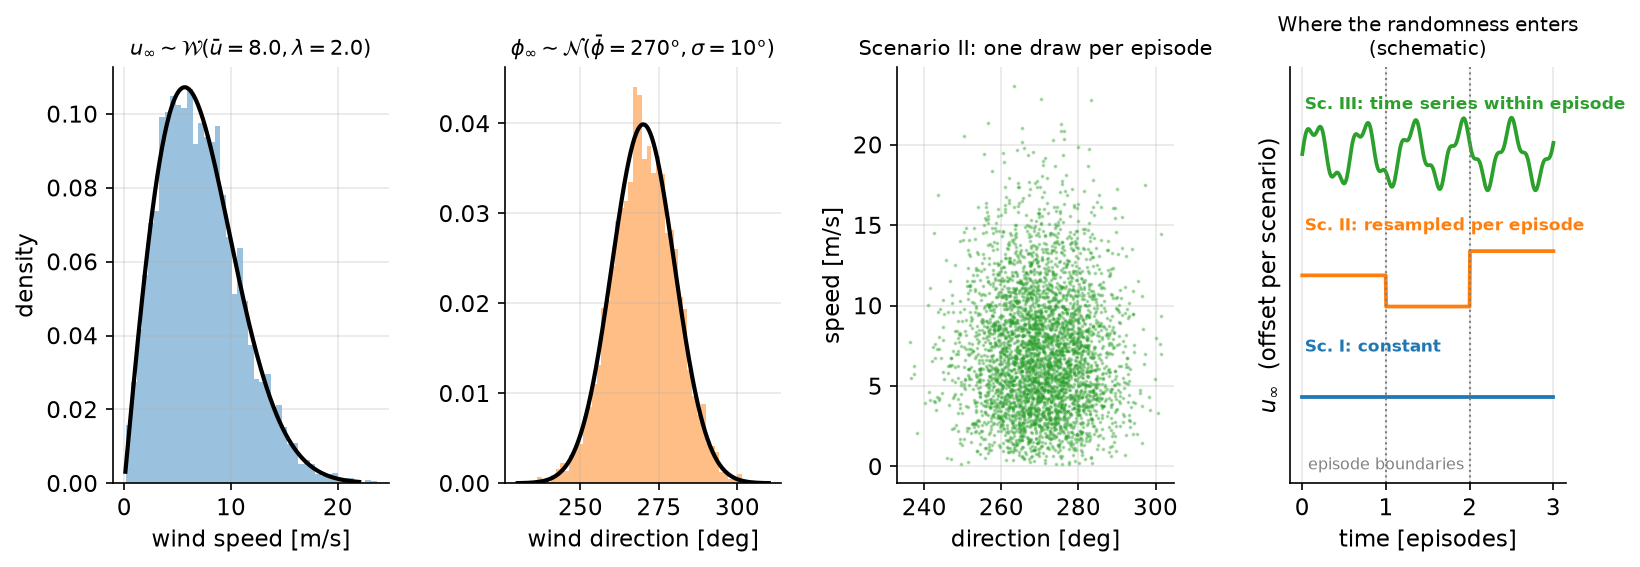
\includegraphics[width=0.99\textwidth]{figs/fig_wind_scenarios.png}
\end{center}
\vspace{1mm}
\footnotesize
\begin{itemize}\setlength\itemsep{2pt}
  \item 前两幅:$\mathcal W(\bar u{=}8,\lambda{=}2)$ 与 $\mathcal N(270^\circ,10^\circ)$ 的采样直方图与解析密度 —— Weibull 的\emph{右偏长尾}正对应“偶发大风”,是风资源评估的标准模型;
  \item 第三幅:场景 II 每回合抽一个 $(\phi_\infty,\wind)$ 点,策略必须在\emph{整片云}上都表现良好,而非只拟合一个工况;
  \item 第四幅(示意):三种场景的差别\emph{只在随机性进入的时间尺度} —— I 恒定 / II 回合间跳变 / III 回合内连续变化。
\end{itemize}
\vspace{1mm}
\centering\footnotesize\color{mygray}
\end{frame}

\begin{frame}{两个后端:静态 FLORIS vs 动态 FAST.Farm}
\small
\begin{center}\renewcommand{\arraystretch}{1.2}
\begin{tabular}{@{}p{0.2\linewidth} p{0.36\linewidth} p{0.36\linewidth}@{}}
\toprule
 & \textbf{FLORIS(静态)} & \textbf{FAST.Farm(动态,OpenFAST)} \\
\midrule
物理保真 & 稳态参数化尾流(高斯/Jensen) & 中保真:动态尾流蜿蜒、合并、逐机组气弹 \\
时间维度 & 无(瞬时稳态) & 有;动作到下游生效存在\emphb{时延} \\
载荷 & 无(仅湍流代理) & 有:叶片面内/面外弯矩、塔筒、传动链 \\
计算代价 & 瞬时(适合海量采样) & 慢(Fortran+MPI,训练需数小时至数天) \\
\bottomrule
\end{tabular}
\end{center}
\vspace{1mm}
\begin{columns}[T]
\column{0.54\textwidth}
\textbf{迁移任务(Transfer Task)}\\
基准把\emph{高保真的 FAST.Farm 当作“真实风场”的代理},用来检验在\emph{低保真 FLORIS 上学到的策略}是否稳健。基准自己的结论:\emph{朴素微调可能不够}——这正是我们做静/动受控对照的直接动机。
\column{0.46\textwidth}
\textbf{代价的量级}\\
FAST.Farm 每个控制步 $\sim\!0.6$\,s,且需 Fortran$+$MPI 驱动;基准报告的训练动辄\emph{一周到两周}机时。FLORIS 则近乎瞬时 $\Rightarrow$ “先静后动”是被算力逼出来的、也是合理的路线。
\end{columns}
\end{frame}

% =====================================================================
\section{我们的工作:真 MAPPO 与静/动对照}
% =====================================================================

\begin{frame}{设计思路:以基准为底座,静态预训练、动态检验}
\small
\emphg{我们目前的实验正是基于 WFCRL 展开的。} 一条“从低保真到高保真”的受控路线:
\begin{enumerate}\setlength\itemsep{2pt}
  \item 用 \textbf{FLORIS 稳态}做快速、大规模策略学习与超参标定(采样便宜);
  \item 用 \textbf{FAST.Farm 动态气弹}做高保真检验,量化“稳态学到的策略/价值在真实动态下是否成立”;
  \item 在\emph{同布局、同算法、同超参}下,把\emphb{后端保真度作为唯一变量},干净分离“静态 vs 动态”本身。
\end{enumerate}
\vspace{1mm}
\begin{columns}[T]
\column{0.5\textwidth}
\textbf{算法:真 MAPPO(CTDE)}
\begin{itemize}\setlength\itemsep{1pt}
  \item $M$ 个\emph{参数共享}局部 actor $\pi(a_i|o_i)$;
  \item 一个吃\emph{全局状态}的集中式 critic $V(s)$;
  \item 连续偏航增量 + GAE + 观测/回报归一化。
\end{itemize}
\column{0.5\textwidth}
\textbf{时序建模:GRU 时序 critic}
\begin{itemize}\setlength\itemsep{1pt}
  \item 动机:FAST.Farm 有\emph{尾流传播时延};
  \item 带记忆的 critic 应在动态后端相对无记忆基线\emph{拉开差距};
  \item \emph{这是一个正在检验的假设}(结果见后)。
\end{itemize}
\end{columns}
\end{frame}

\begin{frame}{第一版“核心结果”,以及它为什么站不住}
\small
同布局 \texttt{Turb3\_Row1}(三机组沿来流对齐,尾流最坏布局),同算法同超参,$20$ 轮 $\times\,64$ 步,末 5 轮均值:
\begin{center}\renewcommand{\arraystretch}{1.2}
\begin{tabular}{@{}lccc@{}}
\toprule
\textbf{实验} & \textbf{整场功率 (MW)} & \textbf{可解释方差} & \textbf{说明} \\
\midrule
静态 MAPPO(FLORIS)      & \textcolor{myblue}{\textbf{5.69}} & $0.362$ & 稳态,价值易学 \\
动态 MAPPO(FAST.Farm)   & \textcolor{myred}{\textbf{2.34}} & $0.191$ & 气弹,价值含噪 \\
动态 GRU-MAPPO          & $1.87$          & $0.056$ & 仅 $18/20$ 轮,见后 \\
\bottomrule
\end{tabular}
\end{center}
\vspace{1mm}
曾据此写下“$2.5\times$ 功率差 $\Rightarrow$ 稳态模型系统性高估功率”。\emphb{这条结论是错的},接下来三页说明怎么发现的、以及正确答案是什么。
\begin{alertblock}{致命的隐藏变量:\texttt{env.reset()} 每次都重抽风况}
\texttt{wfcrl/mdp.py:233--258} —— 每次 \texttt{reset} 都会抽
$\wind \!=\! 8\cdot\mathrm{Weibull}(8)$ 与 $\theta \!\sim\! \mathcal{N}(270^\circ,20^\circ)$,而功率 $\propto \wind^{3}$。
每次训练\emph{只 reset 一次} $\Rightarrow$ 两次实验比的是\textbf{两次风况抽签},不是两种物理。
\end{alertblock}
\end{frame}

% ---------------------------------------------------------------------
\begin{frame}{对照实验(一):$2.5\times$ 完全在抽签噪声范围内}
\begin{center}
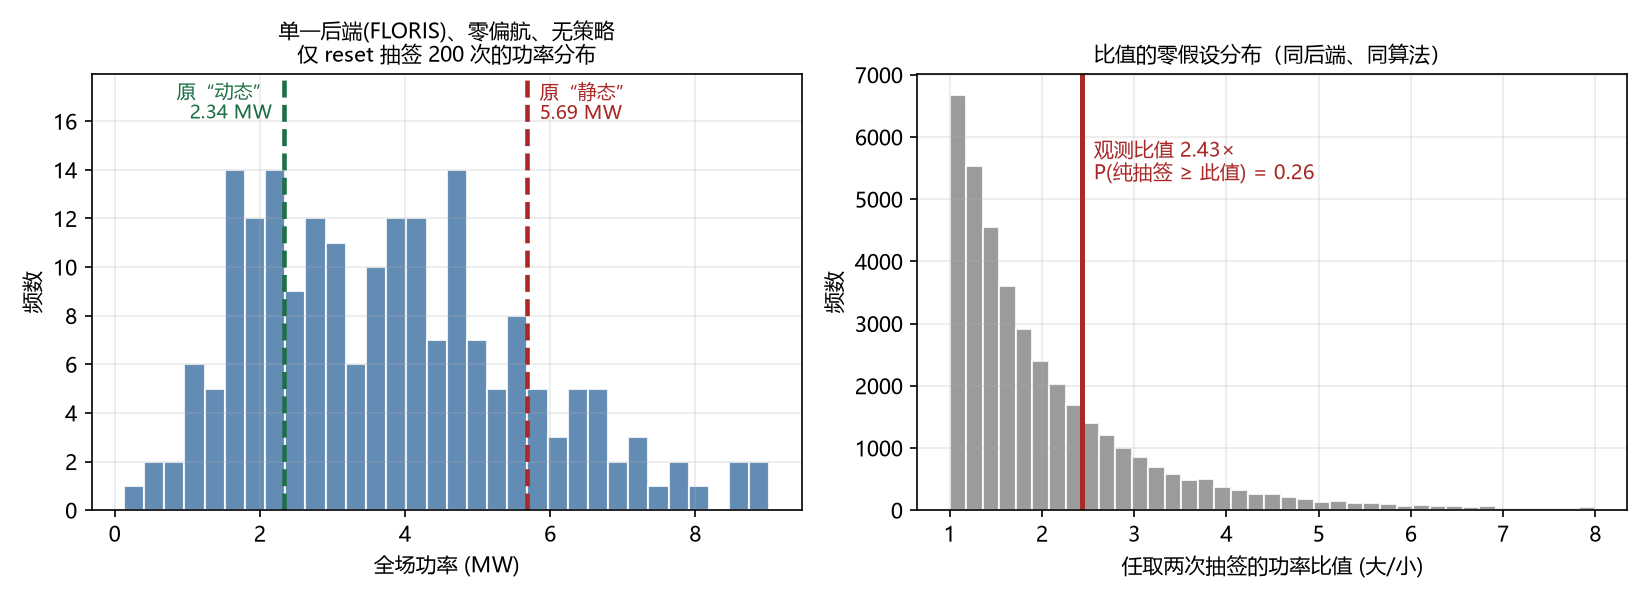
\includegraphics[width=0.96\textwidth]{figs/fig_control_null.png}
\end{center}
\vspace{-2mm}\small
把算法整个移出变量:\emph{同一个后端}(FLORIS)、\emph{零偏航}、\emph{无策略},只反复 \texttt{reset()} 200 次。
\begin{columns}[T]
\column{0.52\textwidth}
\begin{itemize}\setlength\itemsep{1pt}
  \item 来流 $\wind\!:3.49\!-\!9.69$\,m/s,风向 $211^\circ\!-\!316^\circ$;
  \item 整场功率 $0.128\!-\!9.02$\,MW —— \emphb{极差 $70\times$};
  \item 原先那两个观测值\emph{都落在这一个分布内部}。
\end{itemize}
\column{0.48\textwidth}
\begin{alertblock}{零假设检验}
任取两次抽签,功率比值中位数 $1.69$,$P_{90}=3.75$,
$$P(\text{纯抽签比值}\ge 2.43)=\mathbf{0.26}$$
观测值只在噪声分布的第 $74$ 百分位 $\Rightarrow$ \emphb{对“后端差异”零证据力}。
\end{alertblock}
\end{columns}
\vspace{0.5mm}
\centering\footnotesize\color{mygray}
方差分解:$\log P$ 的方差中风速解释 $82.7\%$($\log P$--$\log\wind$ 斜率 $3.25$),剩余方差中风向再解释 $85.1\%$。
\end{frame}

% ---------------------------------------------------------------------
\begin{frame}{对照实验(二):钉死来流后,真正的后端差异}
\begin{center}
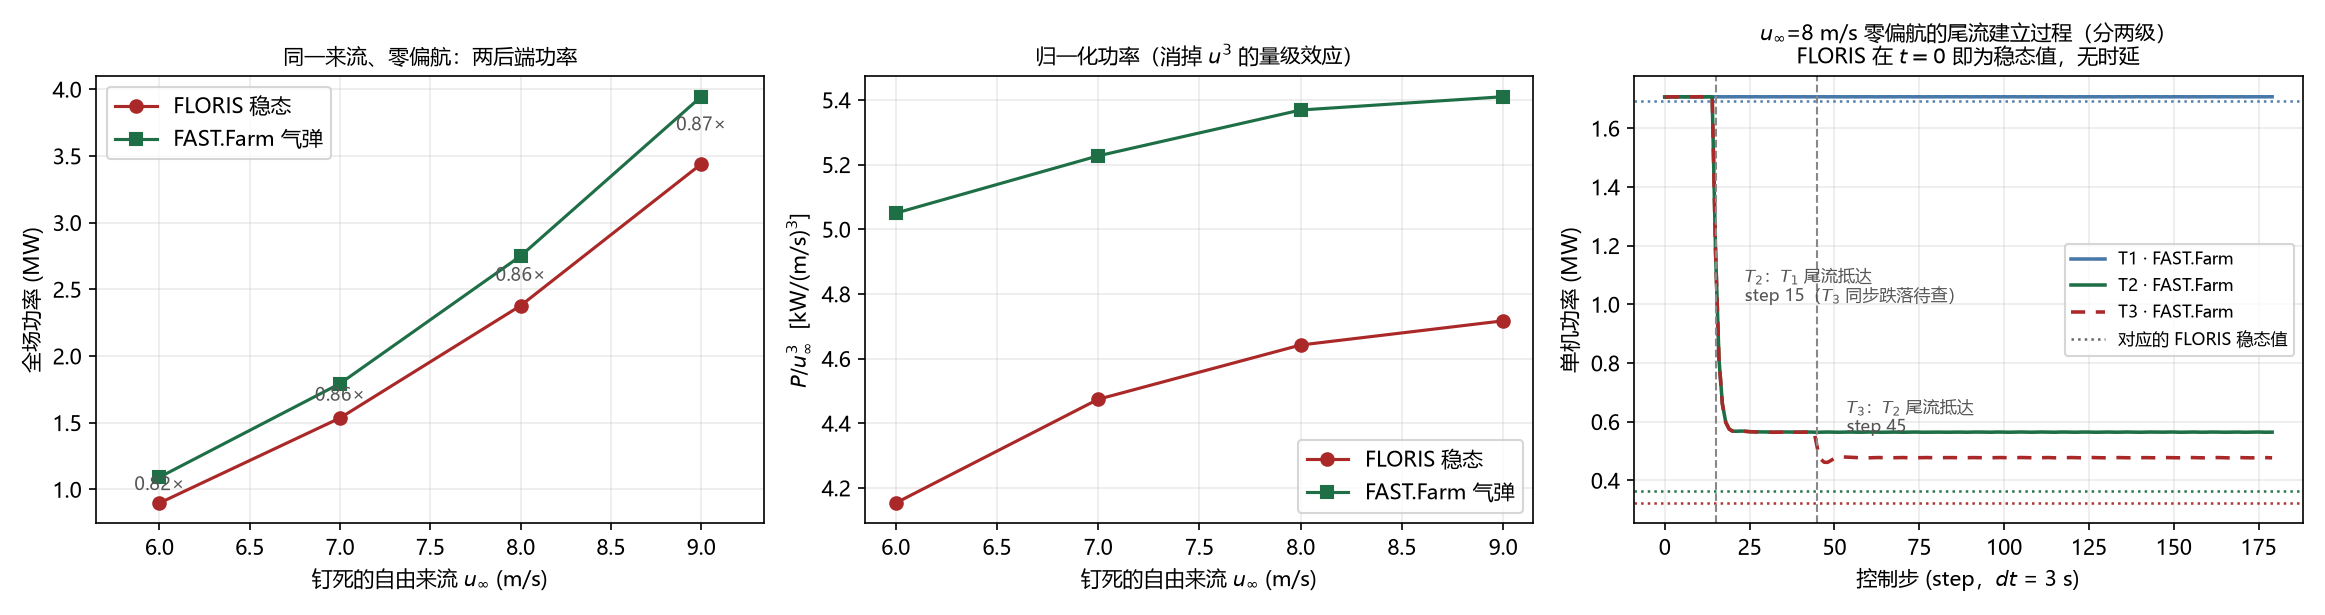
\includegraphics[width=0.99\textwidth]{figs/fig_control_matched.png}
\end{center}
\vspace{-2mm}\footnotesize
\texttt{reset(options=\{"wind\_speed":U,"wind\_direction":270\})} 显式钉死来流(FAST.Farm 侧写入 InflowWind 的 \texttt{HWindSpeed}),零偏航跑到稳态。
\begin{columns}[T]
\column{0.5\textwidth}
\begin{block}{改正后的结论}
同一 $\wind$ 下 FLORIS 比 FAST.Farm \emphb{低 $13\!-\!18\%$},不是高 $143\%$ —— \textbf{方向是反的}。
稳态尾流模型把亏损估计得\emph{更深};气弹里有尾流蜿蜒与湍流掺混带来的动量恢复。
\end{block}
\column{0.5\textwidth}
\begin{itemize}\setlength\itemsep{1pt}
  \item \emph{内部效度}:最上风向 T1 两边一致($\wind\!=\!9$ 时差 $0.3\%$)$\Rightarrow$ 来流确实钉齐;
  \item 差异全在下游:$\wind\!=\!8$ 时 T2 $+55.6\%$、T3 $+47.9\%$;
  \item \emphg{真正的静/动差别在时延}:$\wind\!=\!8$ 下的下游亏损\emph{分两级建立}
        (step $15$ 出现,$T_3$ 于 step $45$ 二级加深,step $53$ 稳态),
        而 FLORIS 在 $t\!=\!0$ 即为稳态 —— \textbf{这才是需要记忆的物理理由}(下页)。
\end{itemize}
\end{columns}
\end{frame}

% ---------------------------------------------------------------------
\begin{frame}{尾流建立的实测时序,与一处归因修正}
\footnotesize
钉死 $\wind\!=\!8$、零偏航、跑 $180$ 步($540$\,s),逐机组功率(MW,$dt\!=\!3$\,s):
\begin{center}\renewcommand{\arraystretch}{1.12}\scriptsize
\begin{tabular}{@{}llcccl@{}}
\toprule
step & $t_{\mathrm{sim}}$ & $T_1$ & $T_2$ & $T_3$ & \\
\midrule
$0\!-\!14$   & $30\!-\!72$\,s   & $1.7070$ & $1.7070$            & $1.7070$            & 三机逐位相同 \\
$15\!-\!19$  & $75\!-\!87$\,s   & $1.7070$ & $1.175\!\to\!0.575$ & $1.174\!\to\!0.575$ & $T_2$/$T_3$ \emph{同步}跌落 \\
$20\!-\!43$  & $90\!-\!159$\,s  & $1.7070$ & $0.5680$            & $0.5676$            & 两者相差 $0.05\%$ \\
$44\!-\!52$  & $162\!-\!186$\,s & $1.7070$ & $0.5642$            & $0.509\!\to\!0.461$ & $T_3$ \emph{单独}二次跌落 \\
$\ge 53$     & $\ge 189$\,s     & $1.7070$ & $0.5645$            & $0.4797$            & 稳态(末 $380$\,s 漂移 $-0.01\%$) \\
\bottomrule
\end{tabular}
\end{center}
\vspace{-1mm}
{\scriptsize\color{mygray}换算:$t_{\mathrm{init}}\!=\!25$\,s、$dt\!=\!3$\,s $\Rightarrow$ \texttt{start\_iter}$\,=\,9$,序列 step $k$ 对应仿真第 $30\!+\!3k$ 秒。}
\vspace{0.6mm}
\begin{columns}[T]
\column{0.44\textwidth}
\begin{block}{两次跌落中归因明确的部分}
\scriptsize
$T_2$ 的第一次跌落:$T_1$ 尾流抵 $T_2$ 需 $504/8\!=\!63$\,s,实测 $75$\,s。\\[0.4mm]
$T_3$ 的第二次跌落:$T_2$ 尾流生于 $75$\,s,$504/5.7\!=\!88$\,s $\Rightarrow$ 预计 $163$\,s,实测 $165$\,s。
\end{block}
\column{0.56\textwidth}
\begin{alertblock}{撤回:“$T_1$ 尾流\emph{同时}抵达 $T_2$ 与 $T_3$”}
\scriptsize
$T_3$ 在 step $15$ 的跌落两条不符:
(i) $T_1$ 尾流抵 $T_3$ 需 $1008/8\!=\!126$\,s(step $32$),而它与 $T_2$ \emph{同步}跌;
(ii) step $20\!-\!43$ 内 $T_2$($4D$)与 $T_3$($8D$)仅差 $0.05\%$ —— 尾流随距离恢复应使 $T_3$ \emph{更高},若已落入 $T_2$ 尾流应\emph{显著更低},等值两者皆不支持。
机理待查,倾向流场初始化填充。\emph{待办}:双机组算例标定 $4D$/$8D$ 亏损。
\end{alertblock}
\end{columns}
\vspace{-1mm}
{\scriptsize\color{mygray}\textbf{工程含义}:前 $15$ 步 $T_2$/$T_3$ 仍在自由来流,偏航对下游无收益、只使 $T_1$ 按 $\cos^3$ 掉功率 —— 该段奖励与目标\emph{反向};动作对 $T_3$ 的完整影响滞后 $\sim\!46$ 步。故回合长度取 $150\!-\!200$ 步并丢弃开头 $46$ 步。}
\end{frame}

% ---------------------------------------------------------------------
\begin{frame}{对照实验(三):钉死来流后重跑 RL,$3$ seed}
\begin{center}
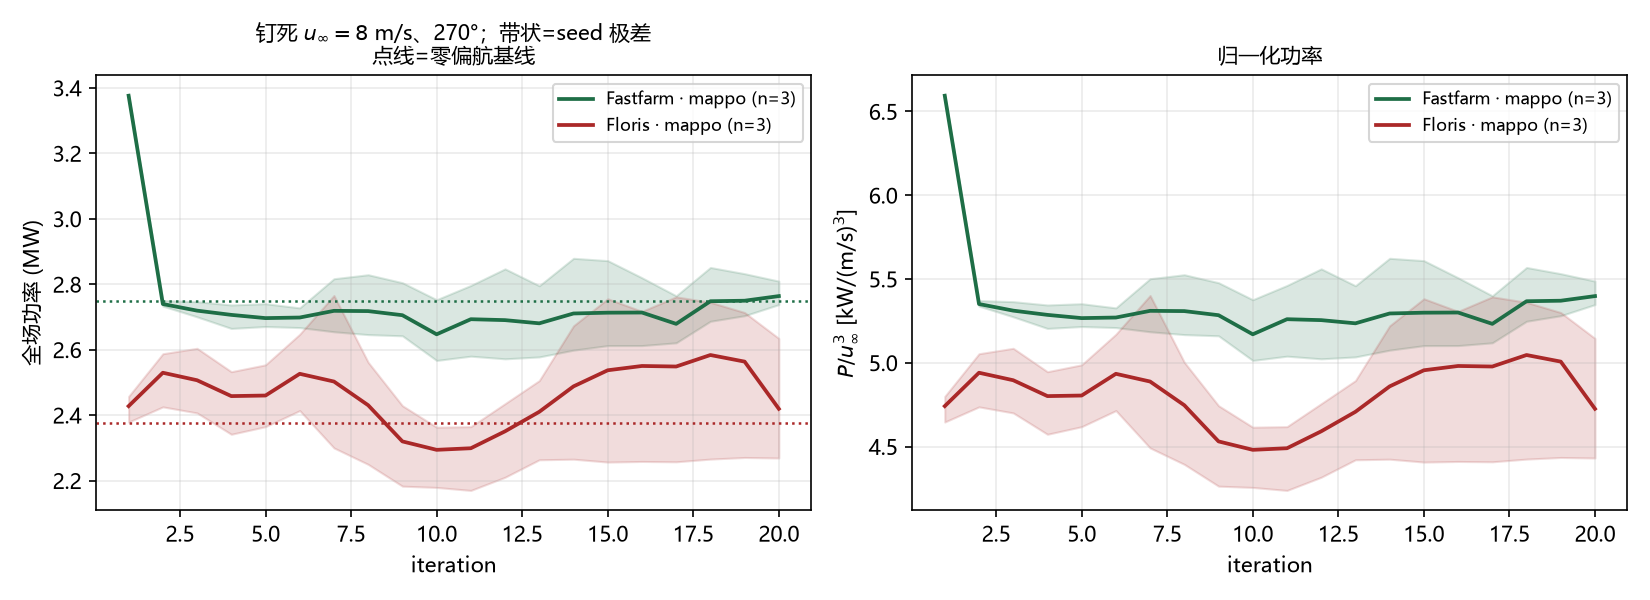
\includegraphics[width=0.90\textwidth]{figs/fig_pinned_seeds.png}
\end{center}
\vspace{-2mm}\footnotesize
\begin{columns}[T]
\column{0.46\textwidth}
\begin{center}\renewcommand{\arraystretch}{1.15}\scriptsize
\begin{tabular}{@{}lccc@{}}
\toprule
 & \textbf{末5轮 (MW)} & \textbf{零偏航} & \textbf{策略增益} \\
\midrule
FLORIS    & $2.533\pm0.191$ & $2.377$ & \textcolor{mygreen}{$+6.6\%$} \\
FAST.Farm & $2.731\pm0.060$ & $2.749$ & \textcolor{myred}{$-0.7\%$} \\
\bottomrule
\end{tabular}
\end{center}
\column{0.54\textwidth}
\begin{itemize}\setlength\itemsep{1pt}
  \item 绝对功率比 $0.928\times$,\emph{方向}与零偏航物理对照($0.865\times$)一致;
  \item \emphb{但 $n{=}3$ 下不能宣称}:两个 seed 区间的间隙只有 $0.0002$\,MW,而 seed 标准差就有 $0.191$\,MW;
  \item 可比的口径是\emph{相对各自零偏航基线}的增益 —— \textbf{$1280$ 步下策略在气弹后端等于没学到}。
\end{itemize}
\end{columns}
\vspace{0.5mm}\centering\scriptsize\color{mygray}
绿色曲线第 1 轮的 $3.38$\,MW 是尾流建立瞬态漏进了统计窗口(前 $15$ 步 $T_2$/$T_3$ 仍在自由来流)。
\end{frame}

% ---------------------------------------------------------------------
\begin{frame}{训练曲线:变量并不只有物理后端}
\begin{center}
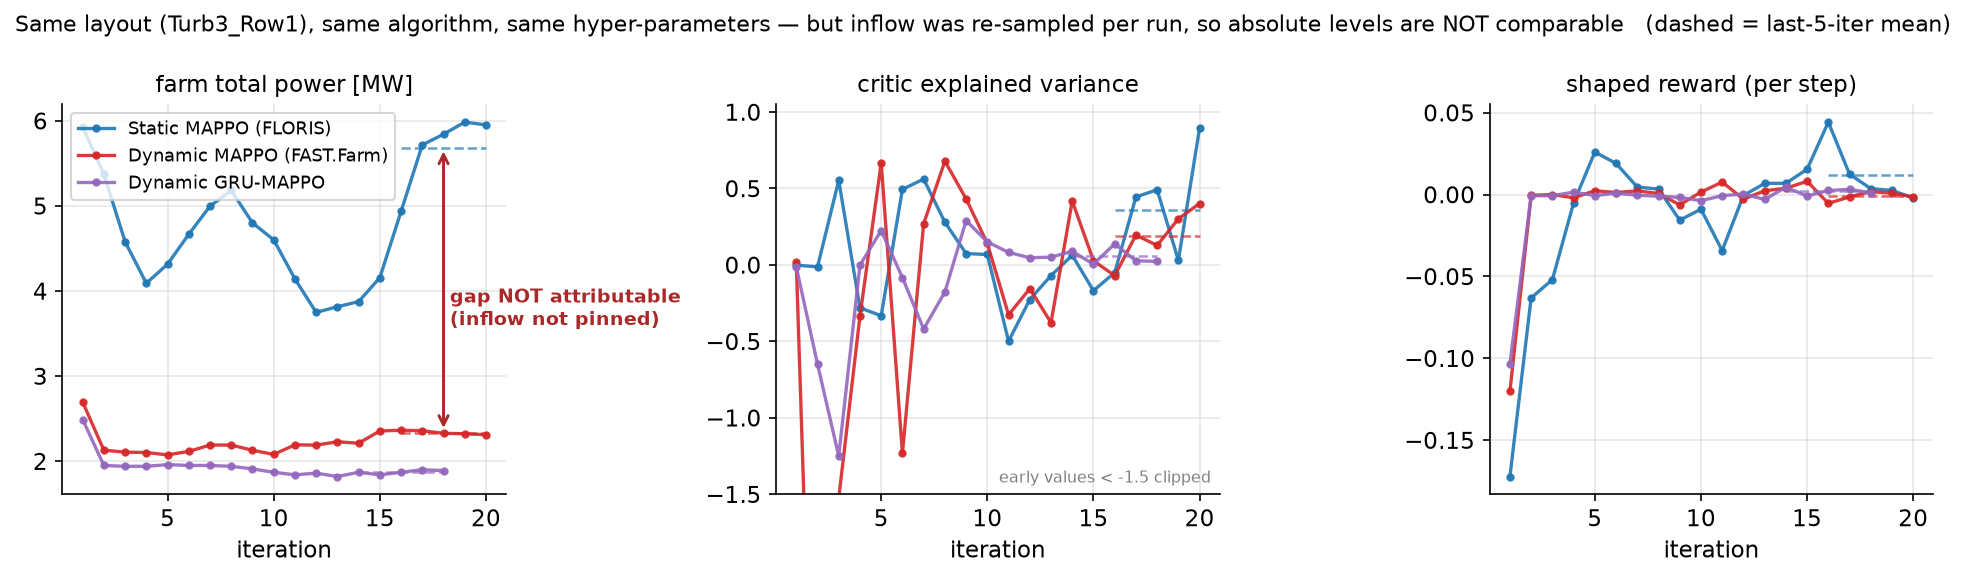
\includegraphics[width=0.99\textwidth]{figs/fig_training.png}
\end{center}
\vspace{-1mm}
\footnotesize
\begin{columns}[T]
\column{0.5\textwidth}
\textbf{读图}
\begin{itemize}\setlength\itemsep{1pt}
  \item \emph{左}:两条功率曲线全程不相交,但\emphb{这个间距不可归因} —— 两次跑各自抽了一次风况,水平高低由抽签决定(见前两页);
  \item \emph{中}:可解释方差 —— 静态末段爬到 $0.36$,动态只有 $0.19$,GRU 路径几乎为 $0$;
  \item \emph{右}:整形奖励经 running-std 归一化后量级很小,主要看趋势。
\end{itemize}
\column{0.5\textwidth}
\begin{alertblock}{两条局限}
\footnotesize
\textbf{(i) 未控变量}:曲线的\emph{绝对高度}含风况抽签,只有\emph{同一条曲线内的趋势}可读。
已把 \texttt{--wind-speed/--wind-direction} 与归一化功率 $P/\wind^3$ 接入训练管线,含策略的受控重跑是下一步。\\
\textbf{(ii) 规模}:本轮只跑 $20\times64=\mathbf{1280}$ 个控制步,基准中 PPO 类是 $\sim\!2\times10^5$ 步,\emph{相差两个数量级} —— 曲线远未收敛。
\end{alertblock}
\end{columns}
\end{frame}

\begin{frame}{GRU 这一轮:结果与根因}
\small
\begin{alertblock}{GRU 这轮\emph{没有赢},但这是\emph{实现缺陷},不是“记忆无用”的结论}
可解释方差 $0.056$(更差),且该轮因外部原因在 $18/20$ 轮被中断、结果由日志抢救。
\end{alertblock}
\textbf{根因}:现有 recurrent 采样阶段每步以 $h_0=\text{None}$ 计算价值 —— GRU 隐状态\emphb{没有跨步携带},GAE 的价值目标\emph{根本没吃到记忆},“时序 critic 的记忆优势”并未被公平行使。
\vspace{1mm}
\begin{block}{要公平检验“动态确实需要记忆”,需改为正规 recurrent PPO}
\emph{有状态 rollout}(隐状态跨步携带并存储)$+$ 更新时\emph{按序列重建做时间反向传播(BPTT)}。这是下一步明确的技术项。
\end{block}
\centering\vspace{1mm}
\emphg{同一处理}:未受控或未验证的观测不作为结论 —— 前面几页的对照实验、以及对尾流归因的那处修正,走的都是这条。
\end{frame}

\begin{frame}{已完成的系统工程 \& 三维数字孪生}
\small
\begin{columns}[T]
\column{0.56\textwidth}
\textbf{工程里程碑}
\begin{enumerate}\setlength\itemsep{2pt}
  \item \emphg{FAST.Farm 动态后端全流程打通}:MS-MPI 运行时 + 官方 ABI 修正,\texttt{mpiexec} 正确 spawn 并驱动;后端无关统一驱动器(PettingZoo AEC $\to$ “一步 = 一个控制步”),妥善排空回合预算避免 MPI 孤儿进程。
  \item \emphg{真 MAPPO 训练管线}:FLORIS / FAST.Farm 两后端均可端到端训练、存 checkpoint、出三联曲线、落 JSON 供叠加对比;GRU 路径已实现(待正规化)。
  \item \emphg{三维数字孪生可视化}:RViz 风格桌面应用(PyVistaQt)。
\end{enumerate}
\column{0.44\textwidth}
\textbf{RViz 风格可视化}
\begin{itemize}\setlength\itemsep{1pt}
  \item 3D 场景可轨道/缩放/平移,机组按真实偏航姿态动画,并可\emphb{直接拖拽机组重定位}(松手即回填 FLORIS 重算尾流,见后两页);
  \item 尾流水平切面随策略\emph{实时刷新};
  \item 侧栏以“通道(等价 ROS topic)”订阅 yaw / power / vibration / wake 遥测;
  \item FAST.Farm 后端:姿态/功率/载荷取\emph{气弹真值},尾流面用\emph{同布局 FLORIS-proxy} 渲染(因 FAST.Farm 不暴露实时流场)。
\end{itemize}
\end{columns}
\vspace{1mm}
\centering\footnotesize\color{mygray}
载荷通道(叶片弯矩)$+$ 运动学(方位角/桨距/挠曲)$\Rightarrow$ 已为后续\emph{多模态感知}预留统一观测总线。
\end{frame}

% ---------------------------------------------------------------------
\begin{frame}{数字孪生现状(一):两个后端的同一套界面}
\vspace{-1mm}
\begin{columns}[T]
\column{0.5\textwidth}
\centering
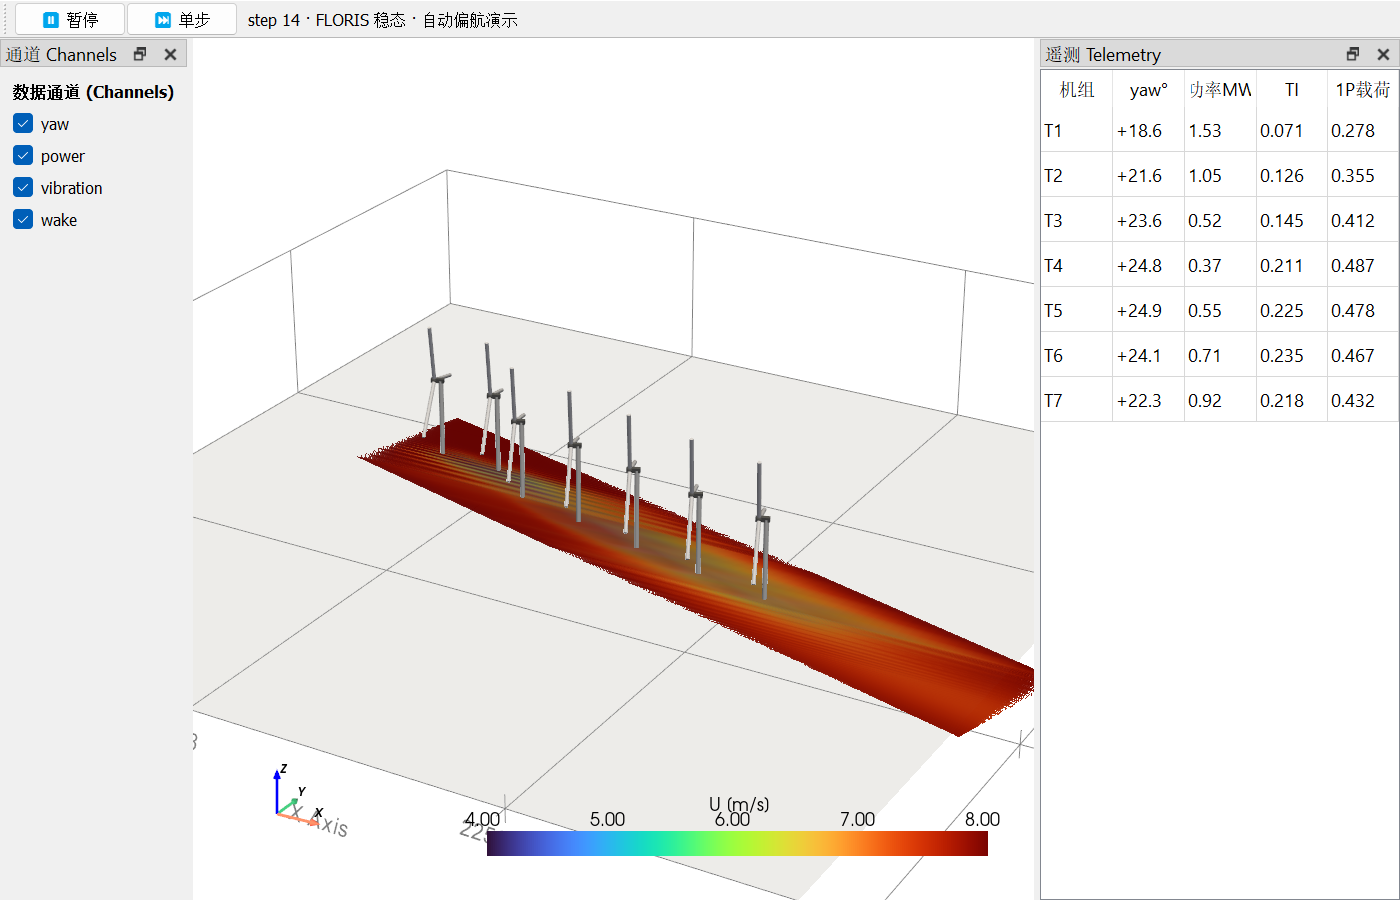
\includegraphics[width=\textwidth]{figs/fig_rviz_overview.png}\\[0.5mm]
{\scriptsize\color{mygray} \textbf{FLORIS 稳态} · Ablaincourt 7 机组 · $\wind=8$\,m/s, $\phi_\infty=285.5^\circ$}
\column{0.5\textwidth}
\centering
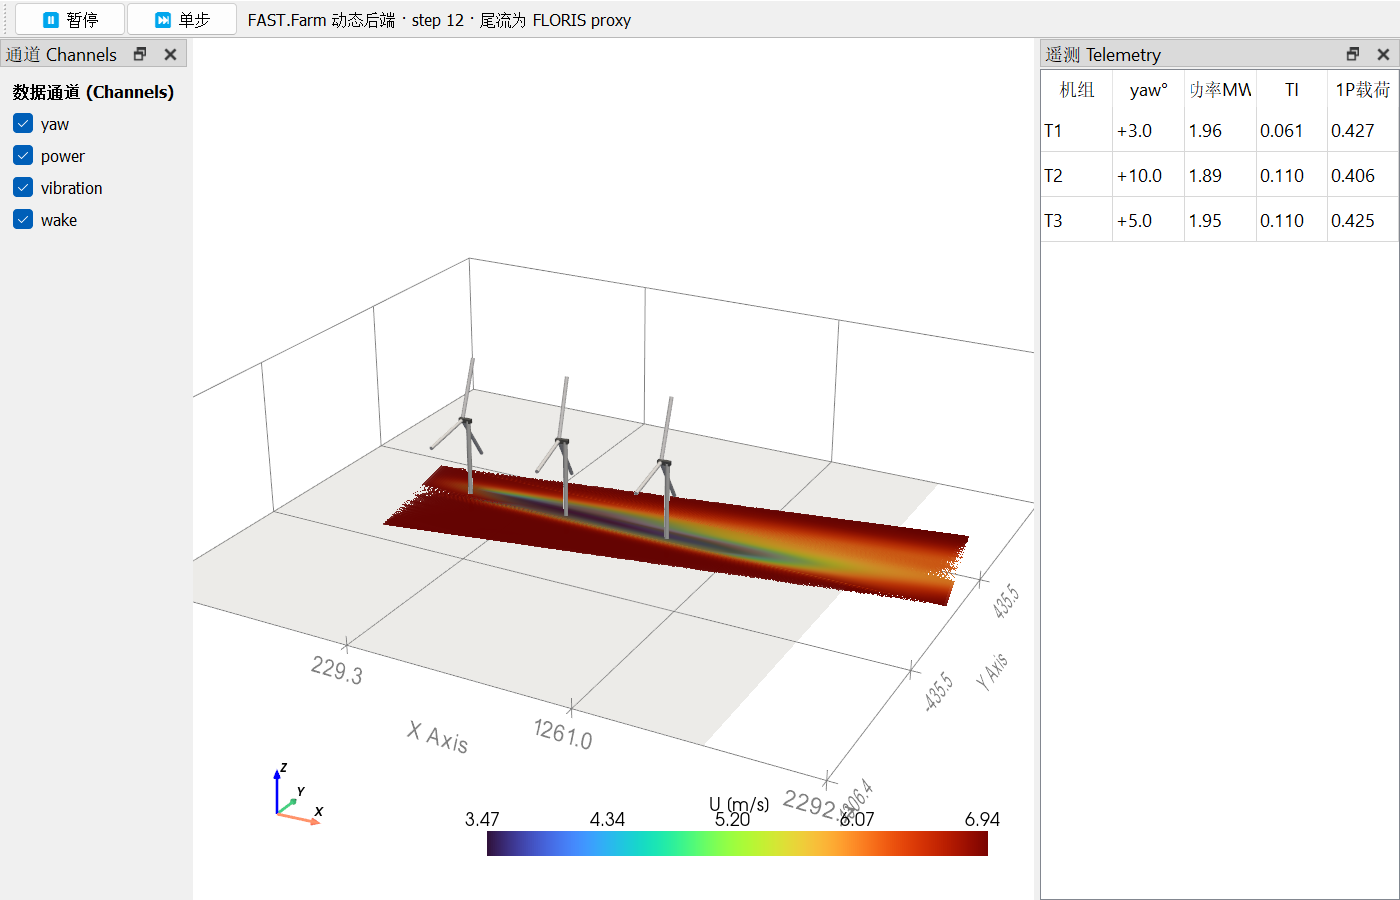
\includegraphics[width=\textwidth]{figs/fig_rviz_fastfarm.png}\\[0.5mm]
{\scriptsize\color{mygray} \textbf{FAST.Farm 动态} · \texttt{Turb3\_Row1} · 姿态/功率/1P 载荷为气弹\emph{真值}}
\end{columns}
\vspace{1mm}
{\footnotesize
左栏 = RViz 的 \emph{Displays}:四条通道(\texttt{yaw/power/vibration/wake})可独立开关;右栏 = 遥测表,每个控制步刷新;
底部色标为轮毂高度水平切面风速。\emphb{同一个窗口类换后端只改数据源}——\texttt{FarmSource} 与 \texttt{FastFarmSource} 是 duck-type 的。
FAST.Farm 那张的尾流面标注为 \emph{FLORIS-proxy}:FAST.Farm 不向 Python 暴露实时流场,只回传每台机组的测量。}
\end{frame}

% ---------------------------------------------------------------------
\begin{frame}{数字孪生现状(二):支持 3D 拖拽 —— 拖完即重算物理}
\vspace{-1mm}
\begin{columns}[T]
\column{0.5\textwidth}
\centering
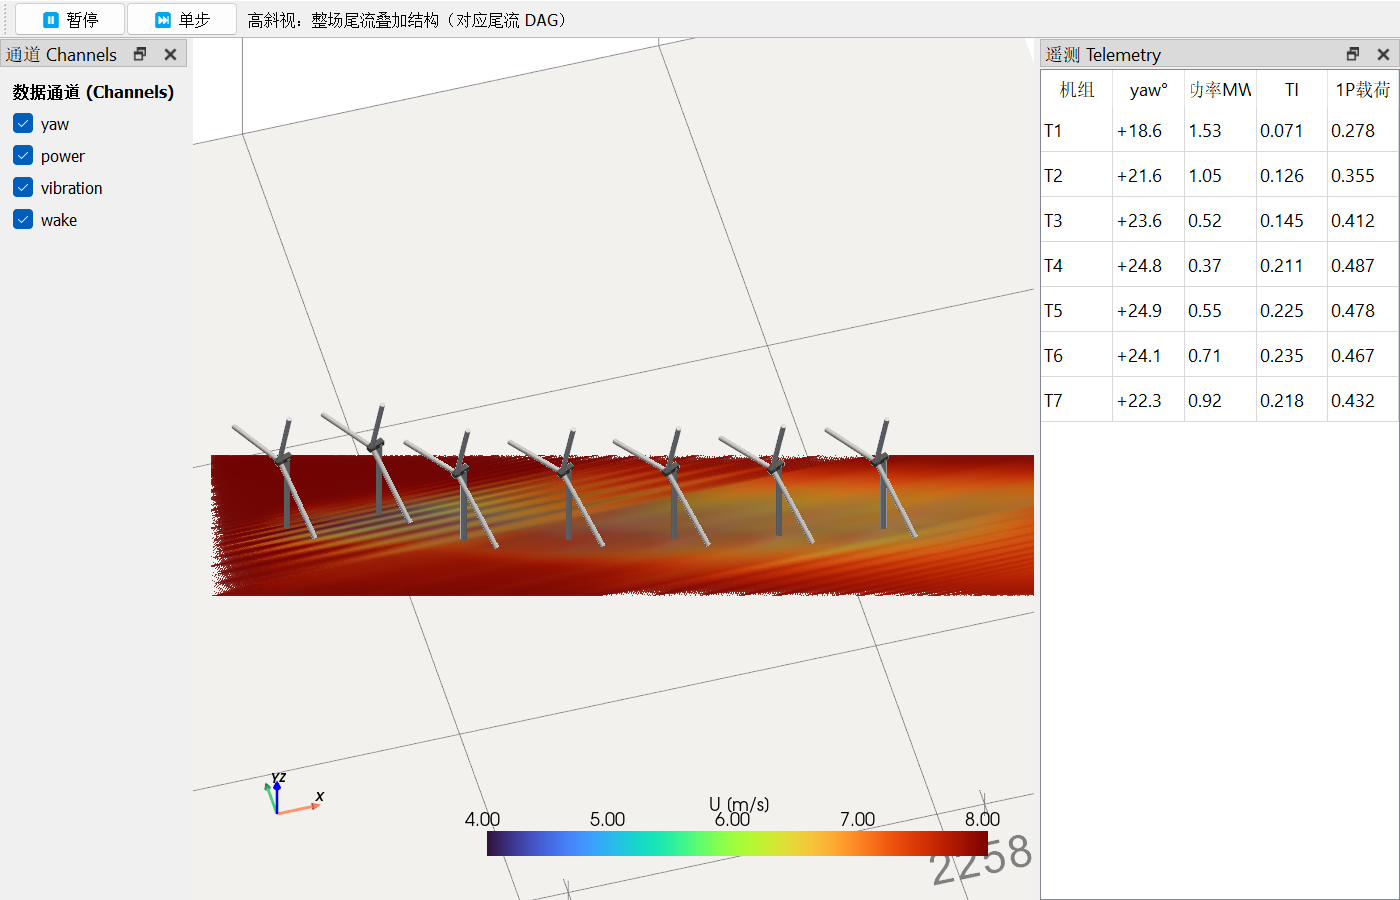
\includegraphics[width=\textwidth]{figs/fig_rviz_topdown.png}\\[0.5mm]
{\scriptsize\color{mygray} 拖拽\emph{前}:七机串列,尾流逐级叠加,合计 \textbf{5.66\,MW}}
\column{0.5\textwidth}
\centering
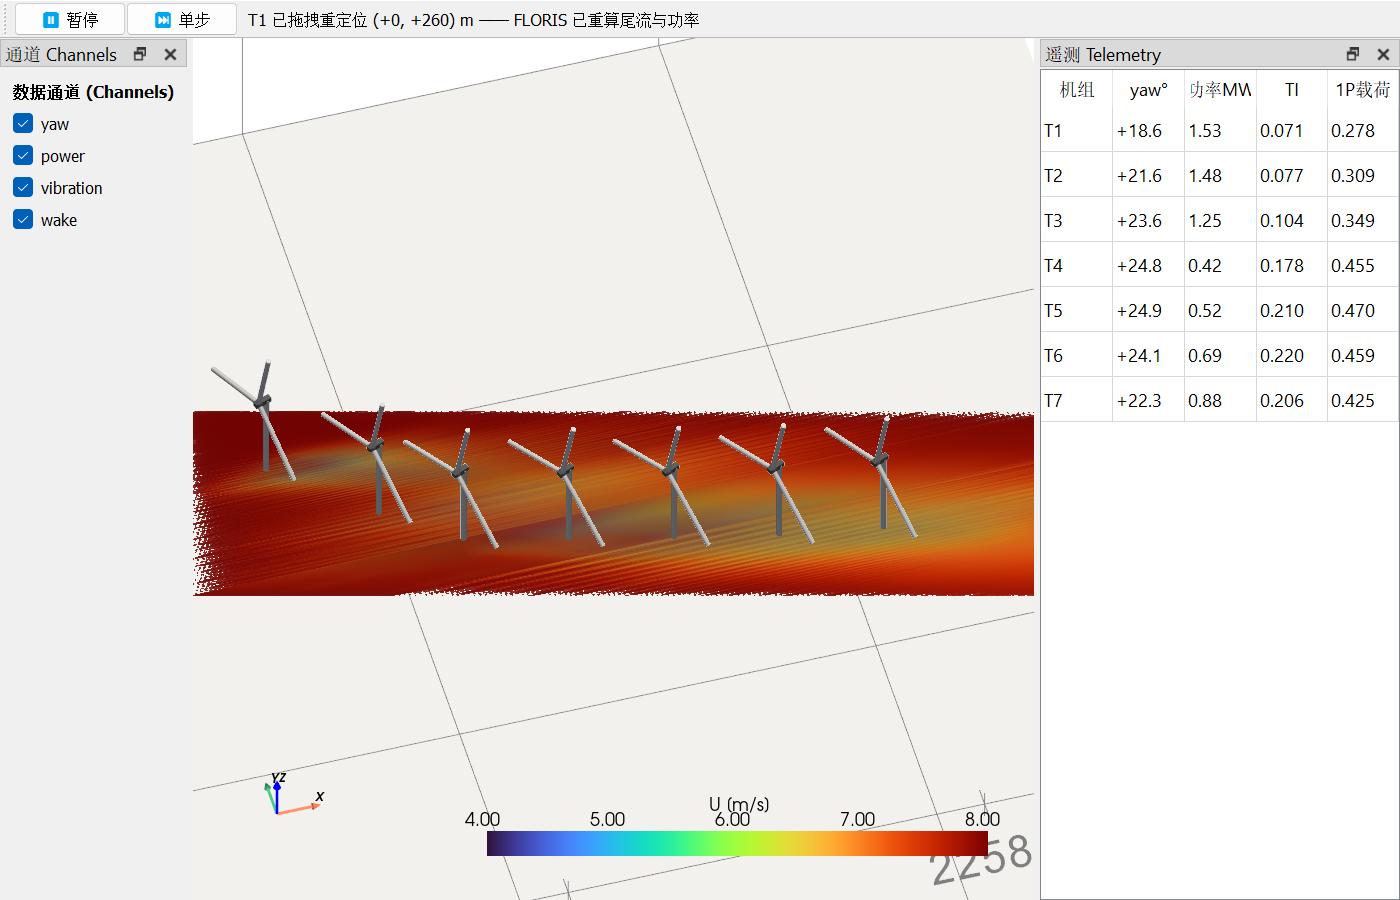
\includegraphics[width=\textwidth]{figs/fig_rviz_drag.png}\\[0.5mm]
{\scriptsize\color{mygray} 把 T1 侧向拖出机列 $(+0,+260)$\,m 后,合计 \textbf{6.77\,MW}}
\end{columns}
\vspace{1mm}
{\footnotesize
两张图\emph{同一相机、同一偏航角}(\,$\gamma=18.6^\circ\!\dots\!22.3^\circ$,只改布局\,):
$P_{T2}: 1.05\!\to\!1.48$, $P_{T3}: 0.52\!\to\!1.25$\,MW,全场 \emphb{$+19.5\%$}。
这正是\emph{尾流 DAG 的边被剪断}的可视化 —— 把上游节点移出下游的入邻域,后代立刻解除亏损。
\emphg{实现}:\texttt{vtkPropPicker} 选中机组 $\to$ \texttt{vtkCellPicker} 在地面求鼠标落点 $\to$ 松手回填 \texttt{floris.reinitialize(layout)} 重算尾流与功率。}
\end{frame}

% ---------------------------------------------------------------------
\begin{frame}{数字孪生:当前短板与丰富化路线}
\small
\begin{columns}[T]
\column{0.47\textwidth}
\textbf{当前短板}
\begin{itemize}\setlength\itemsep{1pt}
  \item 界面仍属\emph{功能原型}:控件只有播放/单步,配色与排版是 Qt 默认;
  \item 尾流只有\emph{一张轮毂高度水平切面},看不到垂直剪切与尾流抬升;
  \item 遥测是\emph{数字表格},没有时序曲线,看不出瞬态;
  \item 拖拽仅 FLORIS 稳态后端可用 —— FAST.Farm 的布局烧死在 \texttt{.fstf} 里,运行中不可迁移。
\end{itemize}
\column{0.53\textwidth}
\textbf{丰富化路线(按性价比排序)}
\begin{enumerate}\setlength\itemsep{1pt}
  \item \emphg{多切面 $+$ 等值面}:叠加若干竖直切面与 $u/\wind=0.9$ 等值面 $\Rightarrow$ 尾流的三维体形,而非一张纸;
  \item \emphg{尾流 DAG 叠加层}:按当前风向实时算出有向边并画在场景里,秩用颜色编码 —— 把理论部分的 $\bar M$ 直接\emph{显示}出来;
  \item \emphg{时序面板}:功率/载荷/奖励滚动曲线 $+$ 回合累计,训练与回放共用;
  \item \emphg{策略对照回放}:贪心 / 训练后策略同屏双视口,差值着色;
  \item \emphb{与训练回路对接}:把它做成 checkpoint 的\emph{查看器}(载入 \texttt{.pt} 即回放),而不是独立脚本;
  \item 远景:接 Isaac Sim/Blender 出 RGB-D,直接喂\emph{多模态 VLM 通道}(见下一节)。
\end{enumerate}
\end{columns}
\vspace{0.5mm}
\centering\footnotesize\color{mygray}
定位:它\emph{不是}演示玩具,而是“物理后端 $\to$ 观测总线 $\to$ 策略”这条链路的\emph{调试与验收工具};前两条已足够支撑本项目的下一步。
\end{frame}

% =====================================================================
\section{系统架构:从脚本到应用}
% =====================================================================

\begin{frame}{目标形态:一个可以“建风场、接数据、训策略、看三维”的应用}
\small
上一节的可视化是\emph{脚本的附属品} —— 布局由 \texttt{env\_id} 反查常量表,通道写死在代码里。
本节把它重构成\emph{应用}:一切由\emphb{场景文件}决定,界面只是它的视图。
\begin{columns}[T]
\column{0.52\textwidth}
\textbf{六层结构}(下层不知道上层存在)
\begin{itemize}\setlength\itemsep{1pt}
  \item \texttt{L0} 物理:FAST.Farm(气弹) / FLORIS(稳态);
  \item \texttt{L1} 场景:一份 YAML $\to$ 机位、机型、来流、控制量;
  \item \texttt{L2} 通道:传感器即订阅源,开关同时管\emph{可见性与采样};
  \item \texttt{L3} 策略 $+$ \emphb{安全约束};
  \item \texttt{L4} 应用外壳:四面板 $+$ 3D 视图,训练跑后台线程;
  \item \texttt{L5} 汇报:本文档与可复现脚本。
\end{itemize}
\column{0.48\textwidth}
\textbf{每层都有独立验收脚本}\\[1mm]
{\footnotesize
\begin{tabular}{@{}ll@{}}
\toprule
层 & 验收判据 \\
\midrule
\texttt{L1} & 改 YAML 坐标,\emph{画面与仿真一起变} \\
\texttt{L2} & 取消订阅 $\Rightarrow$ 采样计数\emph{停住} \\
\texttt{L3} & 指令与环境执行\emph{逐位一致} \\
\texttt{L4} & 训练中事件循环\emph{不卡} \\
\bottomrule
\end{tabular}}\\[1.5mm]
{\footnotesize 判据全部落在\emph{可观测量}上 —— 像素、计数器、毫秒 —— 而不是“没抛异常”。
“没崩”与“对了”是两件事,\emph{只有前者能被自动测到}才是这套脚本的意义。}
\end{columns}
\end{frame}

% ---------------------------------------------------------------------
\begin{frame}{L2 数据通道:订阅是\emph{真的}停采样,保真度必须标出来}
\small
\begin{columns}[T]
\column{0.5\textwidth}
\textbf{通道 $=$ 传感器 $+$ 订阅开关}\\[1mm]
关掉一路通道要\emph{省下真实计算}(激光雷达视线插值、相机离屏渲染),否则“订阅”只是个显示复选框。
验收判据因此写成两条:传感器采样计数\emph{停住},且画面\emph{像素变少}(同一相机下 $47\,419\to30\,450$)。
\vspace{2mm}

\textbf{三档保真度}\\[1mm]
{\footnotesize
\begin{tabular}{@{}lll@{}}
\toprule
档 & 含义 & 可用于 \\
\midrule
\textcolor{mygreen}{\textbf{DIRECT}} & 后端直读 & 奖励、约束、结论 \\
\textcolor{myblue}{\textbf{DERIVED}} & 由直读量导出 & 同上,须注明推导 \\
\textcolor{myred}{\textbf{SYNTH}} & 合成/代理 & \emph{仅}感知层 \\
\bottomrule
\end{tabular}}
\column{0.5\textwidth}
\textbf{为什么这一栏不是 UI 美化}\\[1mm]
FAST.Farm 不向 Python 暴露实时流场,画面上的尾流是\emph{同布局 FLORIS-proxy} —— 稳态解,没有输运时延也没有蜿蜒。
把它当成动态结果去解释,就会把\emph{渲染效果}当成\emph{物理结论}。
\vspace{1.5mm}

因此界面上每一路都带保真度标签与来源说明(悬停可见),\emphb{合成量进不了奖励与约束}。
同理,场景面板专设“\emph{未计入物理}”一栏:地形只进渲染、风向在动态后端不可设 —— 看图的人不会自己知道这些。
\vspace{1.5mm}

\centering\footnotesize\color{mygray}
一张图能否作为证据,取决于它标注了什么,而不是它画得多像。
\end{columns}
\end{frame}

% ---------------------------------------------------------------------
\begin{frame}{L3 安全约束:仿真器会\emph{静默改写}你的动作}
\small
策略输出的不等于机组执行的。三处改写,前两处是限幅,\emphb{第三处是归零}:
\vspace{1mm}
{\footnotesize
\begin{tabular}{@{}p{0.22\textwidth}p{0.30\textwidth}p{0.42\textwidth}@{}}
\toprule
机制 & 出处 & 后果 \\
\midrule
单步增量限幅 & \texttt{mdp.py:300-305} & 偏航 $\pm5^\circ$、桨距 $\pm1^\circ$、转矩 $\pm10^3$\,N·m \\
状态限幅 & \texttt{mdp.py:311-315} & 偏航累计 $[-40,40]^\circ$ \\
\emphb{执行机构占空比} & \texttt{multiagent\_env.py:196-207} & 占空比 $\ge0.1$ 时\emph{整步指令置零} \\
\midrule
桨距是\emph{下界} & \texttt{DISCON.F90:523} & \texttt{PitchRef\,=\,MAX(PitchRef, PitComT)}:低于基线的指令不生效 \\
转矩\emph{完全顶替} & \texttt{DISCON.F90:440} & \texttt{GenTrq\,=\,TorqueRef};动作上界 $2\!\times\!10^4$ 仅为额定 $43\,529$\,N·m 的 \emphb{45.9\%} $\Rightarrow$ 直接下发即超速 \\
\bottomrule
\end{tabular}}
\vspace{1.5mm}

\textbf{最刺眼的一个数}:偏航执行机构速率 $0.3^\circ$/s,占空比上限 $10\%$,控制步 $3$\,s
$\Rightarrow$ 可持续动作仅 $\emphb{0.09^\circ}$/步,而动作空间是 $\pm5^\circ$ —— 相差 \emphb{$55.6\times$}。
\vspace{1mm}

{\footnotesize 不显式建模的后果不是“学得慢”,而是\emph{学到一串从未执行过的动作},且训练曲线上\emph{什么都看不出来}。
约束层把每次改写记成带出处的事件,\texttt{block} 级在界面上标红;验收判据是它的预测与环境的实际执行\emph{逐位一致}(40 步 0 分岔)。}
\end{frame}

% ---------------------------------------------------------------------
\begin{frame}{L3 一个被修正的判据:超速要用\emph{转矩}判,不能用转速}
\small
\begin{columns}[T]
\column{0.5\textwidth}
\textbf{最初的写法}\\[1mm]
转速超过某阈值 $\Rightarrow$ 判超速;更高的阈值 $\Rightarrow$ 判数值发散。
\vspace{1.5mm}

\textbf{为什么它不成立}\\[1mm]
转速并非直接测量,而是由 $\omega=P/(\eta T)$ \emph{反解};
且驱动器已在 $20$\,rpm 处截断。
在截断上限附近设阈值,等于\emph{在自己造的天花板下猜}:$19.9$ 与 $20.1$ 的区别来自截断,不来自物理。
\column{0.5\textwidth}
\textbf{改正}\\[1mm]
判据换成\emphb{发电机转矩}:$|T|<0.3\,T_{\text{额定}}$ 时反解分母趋零 $\Rightarrow$ 判\emph{反解发散};否则判\emph{超速}。
\vspace{1.5mm}

\textbf{并补了反向用例}\\[1mm]
“$19.9$\,rpm $+$ 额定转矩 $\Rightarrow$ 必须判超速”。
没有这一条,“发散”会变成\emph{万能借口} —— 任何异常都能归给数值问题,约束层就失去了报警能力。
\end{columns}
\vspace{2mm}
\centering\footnotesize\color{mygray}
教训可迁移:当一个量是\emph{反解}出来的、且上游已被截断,就不能拿它当判据 ——
要回到\emph{未经处理的那个量}上去。
\end{frame}

% ---------------------------------------------------------------------
\begin{frame}{L4 应用外壳:训练在跑,界面不能卡}
\small
\begin{columns}[T]
\column{0.46\textwidth}
\textbf{硬约束}\\[1mm]
FAST.Farm 一个控制步 $2\!\sim\!3$\,s 墙钟。压在事件循环里,界面就是每 3 秒动一下 —— 拖不动视角、点不了按钮。
\vspace{1.5mm}

\textbf{线程规矩}(违反即白屏或段错误)\\[1mm]
工作线程跑物理与 PPO,只写\emph{纯值}快照;主线程只读快照、只碰 actor。
VTK 的 actor 绑在\emph{创建它的渲染窗口}上,跨线程改变换矩阵是未定义行为。
\vspace{1.5mm}

两个定时器各跑各的:$120$\,ms 取快照喂面板,$33$\,ms 按\emph{真实流逝时间}推进转子相位。
合成一个的话,帧率会被 $3$\,s 的控制步钉死在 $0.4$\,fps。
\column{0.54\textwidth}
\textbf{一次卡顿的定位过程}\\[1mm]
实测最差间隔 \emphb{$3144$\,ms} $\approx$ 恰好一个控制步 $\Rightarrow$ 直觉是“工作线程攥住了 GIL”。
\emph{把间隔拆开量,而不是继续猜}:
\vspace{1mm}
{\footnotesize
\begin{tabular}{@{}lll@{}}
\toprule
分段 & 含义 & 实测 \\
\midrule
\texttt{sleep} 超时 & GIL 被别人占 & $<100$\,ms \\
\texttt{processEvents} & 主线程自己在算 & $\to3144$\,ms \\
\bottomrule
\end{tabular}}
\vspace{1mm}

判据互斥,结论直接:\emph{GIL 无辜},主线程是自己把自己卡住的。逐层下钻找到两处同步计算:
\begin{itemize}\setlength\itemsep{0pt}
  \item FLORIS 稳态解 $0.24\!\sim\!0.36$\,s/控制步;
  \item 叶片柔性变形求解 中位 $192$\,ms(重算 $8000+$ 顶点 $+$ 扫塔间隙搜索)。
\end{itemize}
两者都搬进求解线程,主线程只留数组赋值 $\Rightarrow$ \emphg{$3144\to103$\,ms}。
\end{columns}
\end{frame}

% ---------------------------------------------------------------------
\begin{frame}{Studio:四面板 $+$ 3D,训练进行中}
\vspace{-1mm}
\begin{columns}[T]
\column{0.68\textwidth}
\centering
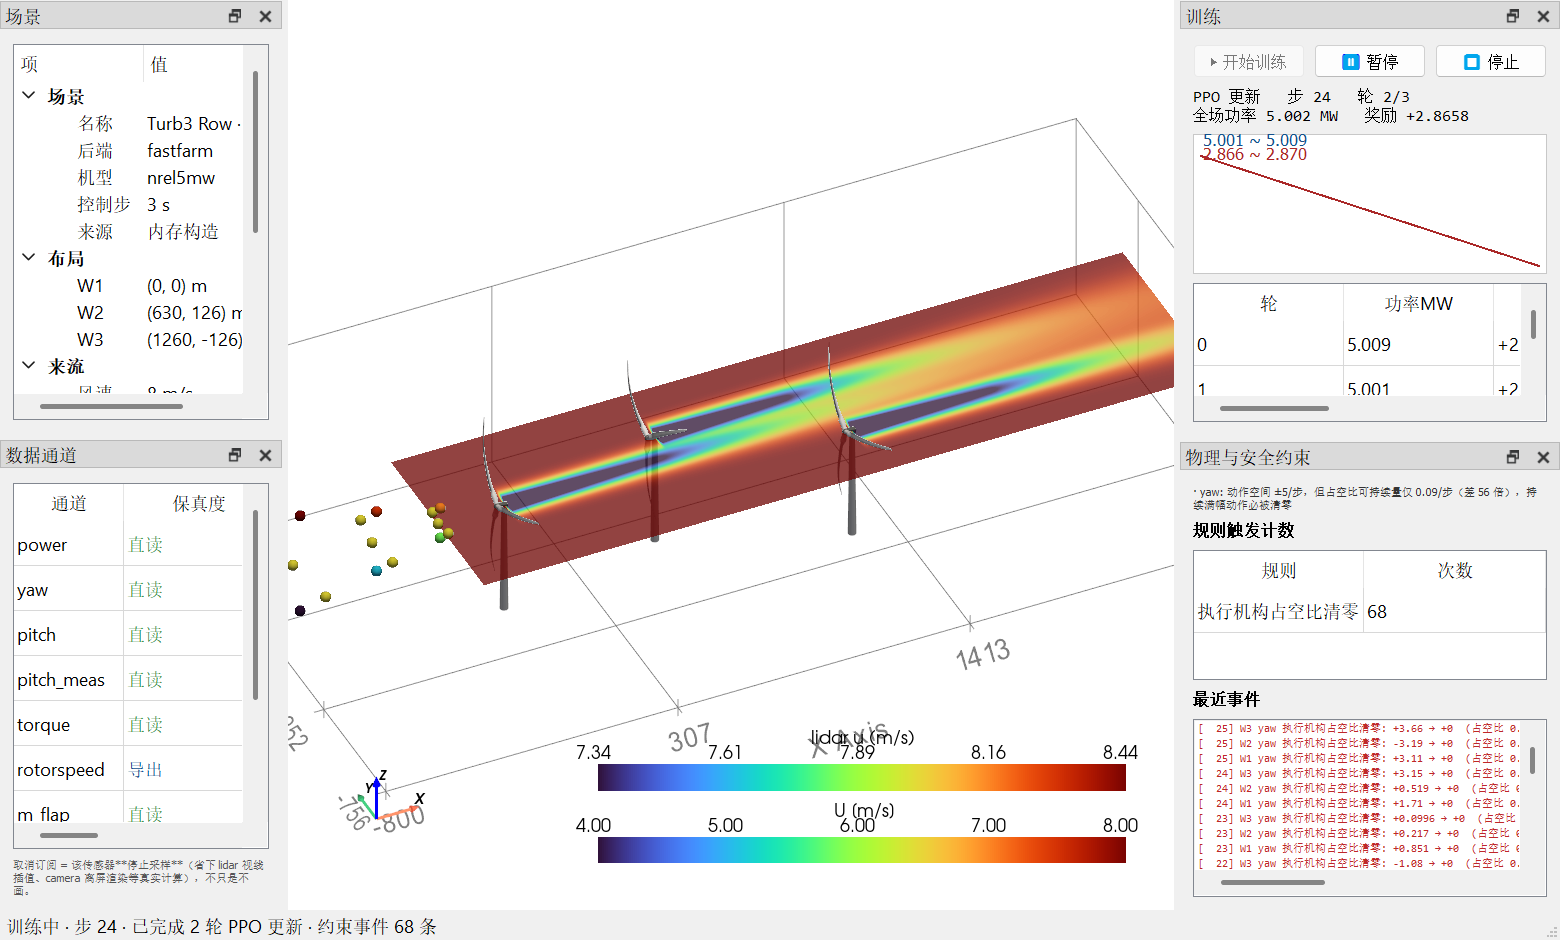
\includegraphics[width=\textwidth]{figs/fig_studio_overview.png}
\column{0.32\textwidth}
\centering
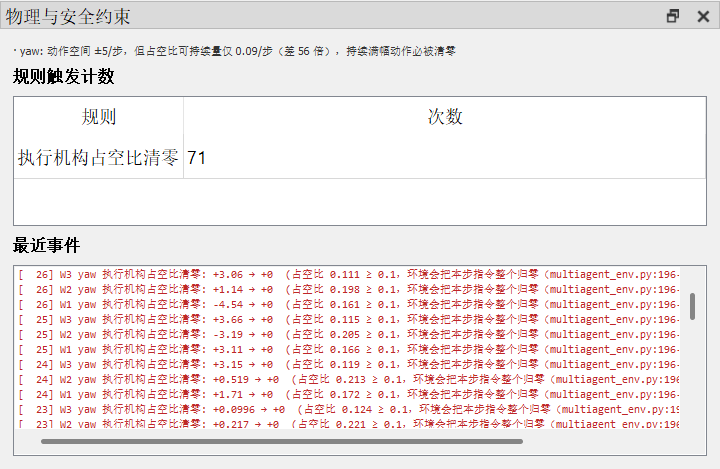
\includegraphics[width=\textwidth]{figs/fig_studio_safety.png}
\end{columns}
\vspace{1mm}
{\footnotesize
左:场景树(含“\emph{未计入物理}”一栏)与通道表(带保真度着色);中:3D 视图,机组按\emph{实测偏航}摆位、按\emph{实测转速}自转;
右:训练面板(功率/奖励双曲线,各自缩放 —— 共用纵轴会把 $\pm3$ 的奖励压成直线)与\emphb{约束事件流}。
右侧特写里每一行都是一次\emph{被环境改写的动作},带占空比数值与源码出处。}
\end{frame}

% =====================================================================
\section{路线图:四阶段目标形态}
% =====================================================================

\begin{frame}{四阶段路线图与当前位置}
\small
\begin{columns}[T]
\column{0.5\textwidth}
\textbf{\textcircled{1} 物理仿真应用}\\
{\footnotesize
Gazebo / Isaac Sim 式界面,消息通道可订阅、开关\emph{立即反映在三维视图上}。\\
\emphg{已有}:场景文件驱动、四面板、通道开关连采样与像素。\\
\emph{待做}:拖拽式场景编辑器、多切面与等值面、尾流 DAG 叠加层。}
\vspace{1.5mm}

\textbf{\textcircled{2} 多模态数据}\\
{\footnotesize
相机、振动、声学、压电;基座模型为视觉语言模型(VLM)。\\
\emphg{已有}:振动/载荷通道取气弹真值,激光雷达点云,统一观测总线。\\
\emph{待做}:RGB-D 渲染管线与真实 VLM 推理。}
\column{0.5\textwidth}
\textbf{\textcircled{3} 有理论依据的控制策略}\\
{\footnotesize
$Q$-学习 / 深度 RL,输出的偏航、桨距、转矩须经\emph{物理与安全约束}校验。\\
\emphg{已有}:MAPPO(集中式 critic,CTDE)$+$ 约束层,改写事件可追溯到源码行。\\
\emph{待做}:约束进入\emph{学习回路}(而非仅事后记录)、疲劳载荷(雨流计数 DEL)入奖励。}
\vspace{1.5mm}

\textbf{\textcircled{4} 市场化}\\
{\footnotesize
按电力市场需求 $+$ 风况联合调度。\\
\emph{待做}:价格信号入观测,收益(而非功率)入奖励,爬坡与备用约束。}
\end{columns}
\vspace{1.5mm}
\centering\footnotesize\color{mygray}
当前位置:\textcircled{1}\,与\,\textcircled{3}\,的\emph{基座}已可运行并有自动验收;\textcircled{2}\,具备数据通道但缺视觉模态;\textcircled{4}\,尚未开始。
\end{frame}

% =====================================================================

\begin{frame}{下一步:面向多模态 VLM$+$RL 的风机智能控制}
\small
在已打通的“物理 $+$ MARL $+$ 数字孪生”基座上,把控制升级为\emph{多模态感知—决策}问题。
\begin{columns}[T]
\column{0.5\textwidth}
\textbf{数字孪生协同仿真架构}\\
保持\emph{物理层不动},在其周围加装:
\begin{itemize}\setlength\itemsep{1pt}
  \item \emph{SCADA 合成}($u_i,\phi_i,P_i,y_i,p_i,\tau_i$,现成);
  \item \emphb{振动/IMU 通道}(叶片弯矩、加速度 —— FAST.Farm“免费”给的最强多模态通道);
  \item \emph{三维渲染器}(Isaac Sim/Blender,运动学驱动 NREL 5\,MW 网格 $\to$ RGB/深度图 —— 唯一需新增工程的模态)。
\end{itemize}
\column{0.5\textwidth}
\textbf{VLM 的四个价值点}
\begin{enumerate}\setlength\itemsep{1pt}
  \item \emph{感知增强}:识别 SCADA 看不到的可视条件(尾流蜿蜒、叶片结冰/损伤);
  \item \emph{高层协调器}:在尾流 DAG“场景图”上推理,提偏航意图,底层 MARL 执行;
  \item \emph{语言条件奖励}:用自然语言设定 $\alpha$(“今天优先保护前排叶片寿命”);
  \item \emph{巡检智能体}:消费相机+振动谱,闭合“控制—运维”回路。
\end{enumerate}
\end{columns}
\vspace{1mm}
\centering\footnotesize\color{mygray}
更远景:嵌入\emph{三层自进化架构}(ICL 秒级纠偏 / LoRA 小时级情景记忆 / RL 天级程序性记忆),在安全约束下在线进化。
\end{frame}

% =====================================================================
\begin{frame}{总结}
\small
\begin{columns}[T]
\column{0.5\textwidth}
\textbf{一条完整的叙事弧线}
\begin{enumerate}\setlength\itemsep{2pt}
  \item \emphb{理论}:Dec-POMDP $\to$ TI-Dec-MDP 重构 $\to$ 部分可观即马尔可夫噪声 $\to$ 光滑均衡;
  \item \emphb{收敛}:多尺度 $Q$-学习,$\beta\le1-K$;尾流 DAG $\to$ NetworkMQL;随机逼近 ODE 方法;
  \item \emphb{基准}:WFCRL 双后端、奖励设计、IPPO/MAPPO/QMIX;
  \item \emphg{我们}:真 MAPPO 双后端管线;\emph{受控}的静/动物理对照;GRU 局限已界定;
  \item \emphg{未来}:多模态 VLM$+$RL 数字孪生。
\end{enumerate}
\column{0.5\textwidth}
\textbf{核心贡献与信息}
\begin{itemize}\setlength\itemsep{3pt}
  \item 把\emph{理论保证}(为何独立学习能work)与\emph{工程现实}(连续动作、深度网络、高保真动态)之间的\emph{鸿沟},做成了\emph{可测量的实验};
  \item \emphb{头条发现}:静/动的本质差别\emph{不在功率量级,而在尾流建立的时延与分级}(下游亏损分两级建立,动作对 $T_3$ 的完整影响滞后 $\sim\!46$ 个控制步,而控制步只有 $3$\,s)—— 这是\emph{记忆型策略}的直接物理依据;
  \item \emphb{方法论}:基准的 \texttt{reset} 每次重抽风况且 $P\!\propto\!\wind^3$,单次抽签足以制造 $2.4\times$ 的假效应 —— 已定位、已钉死、已改正结论;
  \item 打通了\emph{“稳态预训练 $\to$ 动态检验 $\to$ 三维多模态数字孪生”}的可复现链路。
\end{itemize}
\end{columns}
\vspace{2mm}
\centering
{\color{myblue}\Large 谢谢!\quad\normalsize 欢迎提问与批评}
\end{frame}

% ---------------------------------------------------------------------
\begin{frame}[allowframebreaks]{主要参考文献}
\footnotesize
\begin{thebibliography}{9}
\bibitem{partial} C.~Bizon Monroc, A.~Bu\v{s}i\'c, D.~Dubuc, J.~Zhu.
  \emph{Multi-agent reinforcement learning for locally observable cooperative systems with acyclic dependence structure.}
  预印本 (HAL hal-04560319v2), 2025.\\ {\color{mygray}—— 理论主线起点:TI-Dec-MDP、部分可观即马尔可夫噪声、多尺度 $Q$-学习收敛与 NetworkMQL 的完整证明。}
\bibitem{wfc} C.~Bizon Monroc, A.~Bu\v{s}i\'c, D.~Dubuc, J.~Zhu.
  \emph{Wind farm control with cooperative multi-agent reinforcement learning.}
  Workshop on Aligning RL Experimentalists and Theorists (ARLET), 2024.\\ {\color{mygray}—— Q-学习落地:多尺度 $Q$-学习在 16 机组风场的经验验证。}
\bibitem{wfcrl} C.~Bizon Monroc, A.~Bu\v{s}i\'c, D.~Dubuc, J.~Zhu.
  \emph{WFCRL: A Multi-Agent Reinforcement Learning Benchmark for Wind Farm Control.}
  NeurIPS 2024, Datasets and Benchmarks Track.\\ {\color{mygray}—— 实践指导:FLORIS/FAST.Farm 双后端、奖励设计、IPPO/MAPPO/QMIX 基线。}
\bibitem{borkar} V.~S.~Borkar.
  \emph{Stochastic approximation with two time scales.}
  Systems \& Control Letters, 29(5):291--294, 1997.
\bibitem{kushneryin} H.~J.~Kushner, G.~G.~Yin.
  \emph{Stochastic Approximation and Recursive Algorithms and Applications.} Springer, 2003.
\bibitem{ppo} J.~Schulman, F.~Wolski, P.~Dhariwal, A.~Radford, O.~Klimov.
  \emph{Proximal Policy Optimization Algorithms.} arXiv:1707.06347, 2017.
\end{thebibliography}
\end{frame}

\end{document}
